
\documentclass[12pt,letterpaper,oneside]{book} 
 

\usepackage[headings]{thesisstyle}
\usepackage[T1]{fontenc}
%\usepackage{times}
%\usepackage{mathptm}


% \usepackage{color}

\usepackage{amsfonts,amsthm,amssymb,amsmath} 
\usepackage[pdftex]{graphicx} 
\DeclareGraphicsRule{.pdftex}{pdf}{.pdftex}{} 
\usepackage{setspace} 
\usepackage{url}
\usepackage{verbatim} 
\usepackage{algorithmic} 
\usepackage{algorithm} 
\usepackage{fancyhdr} 
\usepackage{mathtext} 
\usepackage{mathrsfs} 
\usepackage{amsfonts} 


%COMPILE AT SCHOOL OR INSTALL PACKAGE
\usepackage[hang,font=small,labelfont=bf,textfont=it]{caption}

%\pagestyle{fancy} 


%%temp
%\lhead{Sam Bassett} 
%\rhead{\today} 
%\setlength{\headheight}{15pt}
%\setlength{\topmargin}{.25in} 
%\setlength{\leftmargin}{1.25cm} 
%%\setlength{\evensidemargin}{3.17cm} 
%%\setlength{\oddsidemargin}{3.17cm}  
%%\setlength{\textheight}{8.25in} 
%\setlength{\textwidth}{6in} 
%\setlength{\footskip}{.4in} 
%\setlength{\headwidth}{\textwidth}  
 %%endtemp



\title{Low memory graph traversal} 
\author{Samson Bassett} 
\qualifications{B.Sc. Hon., Thompson Rivers University, 2007.}

\degree{Master of Science}
\department{Mathematics}
\submitdate{July 2010}  
\thesistype{thesis}   % standard is "thesis"
\entity{Department}   % standard is "Department"
\copyrightyear{2010}      % standard is current


% If you want to grant the copyright instead of reserving it,
% uncomment the next line!
%\grantcopyright   


\chair{Dr. Ralf Wittenberg}
\committee{Dr. Ladislav Stacho}

%\noindent Senior Supervisor

\committee{Dr. Petr Lisonek}

%\noindent Supervisory Committee


\committee{Dr. Binay Bhattacharya}

%\noindent Internal Examiner

\approvaldate{August 23rd, 2010}

\abstract{We provide two traversal algorithms.  In the second chapter, we demonstrate that there exists 
a local orientation for any anonymous, $P_3$-free graph $G$ with $\delta(G)\ge 2$, such that we can periodically traverse the graph with 
period $\pi(n)\le 2n-2$; this matches the lower bound for the period for general graphs.  In the third chapter, we provide a traversal 
for labelled graphs given that they satisfy two properties, which we define.  The properties that 
we define and use are inspired by the properties of geometric planar graphs. }




\newcommand{\procedure}{\textbf{procedure}}
\newcommand{\mintail}{\textbf{mintail}}
%\newcommand{\twopath}{\textbf{twopath}}
\newcommand{\rev}{\textbf{rev}}
\newcommand{\suc}{\textbf{succ}}
\newcommand{\pred}{\textbf{pred}}
\newcommand{\prev}{\textbf{prev}}
\newcommand{\next}{\textbf{next}}
\newcommand{\nextright}{\textbf{nextright}}
\newcommand{\cwalk}{\textbf{cwalk}}
\newcommand{\entry}{\textbf{entry}}
\newcommand{\parent}{\textbf{parent}}
\newcommand{\ismin}{\textbf{ismin}}
\newcommand{\head}{\textbf{head}}
\newcommand{\tail}{\textbf{tail}}
%\newcommand{\loc}{\textbf{loc}}
%\newcommand{\locv}{\textbf{locv}}
%\newcommand{\drop}{\textbf{drop}}
%\newcommand{\bblank}{\textbf{blank}}
%\newcommand{\virtual}{\textbf{virtual}}

\newcommand{\key}{\textbf{key}}
\newcommand{\closer}{\textbf{smaller}}
\newcommand{\smaller}{\textbf{smaller}}
\newcommand{\xcor}{\textbf{x}}
\newcommand{\ycor}{\textbf{y}}
\newcommand{\zcor}{\textbf{z}}
\newcommand{\sx}{\textbf{sx}}
\newcommand{\sy}{\textbf{sy}}
\newcommand{\sz}{\textbf{sz}}
%\newcommand{\entryport}{\textbf{ entryport}
%\newcommand{\fillempty}{\textbf{ fillempty}

\newcommand{\degr}{d} 
\newtheorem{theorem}{Theorem}[section] 
\newtheorem{lemma}[theorem]{Lemma} 
\newtheorem{obs}[theorem]{Observation} 
\newtheorem{proposition}[theorem]{Proposition} 
\newtheorem{definition}[theorem]{Definition}
\newtheorem{corollary}[theorem]{Corollary} 
%\newtheorem{procedure}[theorem]{procedure} 
 


















\begin{document} 
\frontmatter
\maketitle


\chapter[Dedication]{}  % writes `Dedication' into table of contents,
			% but not on actual page 
\begin{center}
\Large
\emph{Dedicated to Rikki.}
\end{center}


% end of dedication
%\begin{comment}
\chapter{Acknowledgments}


\begin{center}
\Large
\vspace{2cm}
\emph{To Mr. Hanson, who taught me how to learn.  }
\newline
\newline
\newline
\emph{To Dr. Rick Brewster, who showed me the}\newline
\emph{ computational side of mathematics.  }
\newline
\newline
\newline

\emph{Finally, to Dr. Ladislav Stacho, whose endless patience, dedication, and support made this possible.  }

\end{center}
%\end{comment}
% end of acknowledgements


\newpage
\addcontentsline{toc}{chapter}{\contentsname}
 \tableofcontents


\newpage
\addcontentsline{toc}{chapter}{\listfigurename}
\listoffigures
\newpage


\mainmatter
\chapter{Introduction} 
 
%** edit and update, include references to geometric traversal, make sure there is less redundancy in the indroduction of that subsection,
%*add mention of extension of periodic traversal to general graphs - after it is written.

%exploration vs traversal vs hamiltonian cycle.  use citations at the bottom.

%unlabeled: bfs, dfs, random walk, geometric: planar, quasiplanar

%unlabelled: broadcasting periodic: 2n-2, 10n, 4n-O1 conjecture, 4n, 3.75n. then our result.

\section{Motivation and Background}
In this thesis we consider the \emph{graph traversal} problem, which asks for a route on a graph that visits every vertex, after 
starting from an arbitrary vertex.  We are interested in finding a graph 
traversal algorithm, which starts at any given initial vertex, and moves between adjacent vertices, to eventually visit 
every vertex of the graph at least once.   
This problem is similar to than the problem of \emph{route discovery}, or $st$-\emph{connectivity}, 
which wants to find a route between two given vertices $s$ and $t$.  
Clearly, a solution to the graph traversal problem will guarantee a route between any two vertices, and hence a graph traversal can 
also be used to solve $st$-connectivity.  %Furthermore, if such a route can be found between any pair of vertices $s$ and $t$, 
%then this route can be extended to contain all vertices of the graph.  
Note 
that in general, algorithms for these problems will not find the shortest possible paths.  Some variations of the graph traversal include 
additionally requiring 
the route to end on the same vertex it started on, or visit every edge of the graph.  %A more difficult version of this problem 
%is the universal traversal sequence problem \cite{FR}, which we define below.  


The model of computation used for a graph traversal is 
typically some type of mobile agent, or robot, that only knows local information of the graph, (i.e., it cannot 
see the entire graph).   
These robots are usually defined as finite automata.  The robot visits exactly one vertex at a time, called the 
current vertex of the robot, and may put a pebble on the vertex (if it has pebbles).  
The running time (sometimes called time complexity) of a traversal algorithm is an 
upper bound on the number of edges the robot visits during the traversal.  
Hence the running time of any traversal algorithm has the trivial lower bound of $\Omega(n)$ for 
an $n$ vertex graph.  The memory used by the robot, (sometimes called space complexity), which is measured in bits, includes the 
states, as well as any other memory (such as a bit representation of pebbles) used by the particular robot.  For example, a 
finite automaton with $q$ states uses at least $\log q$ bits of memory, (since it is in one state at a time, and each 
state has a label of $\log q$ bits).  In the following, we further discuss the memory of the robot, 
depending on the context.  

Graph traversal problems come in two categories, based on whether or not the robot can distinguish between vertices of the graph.  
We say the graph is a \emph{labelled} graph, 
if each vertex has a unique label, (that is readable by the robot).   For example, 
we can use labels $1,2,\ldots,n$ for a graph with $n$ vertices.  
Hence, for labelled graphs, there is a trivial memory lower bound of $\Omega(\log n)$ bits, 
since $\log n$ bits are required to represent an integer no larger than $n$, (and since the number of states in the finite 
automaton is constant).  If every vertex of the graph 
does not have a unique label, we say the graph is \emph{anonymous}.  
In anonymous graphs, we allow edges at an incident vertex to be distinguishable from one another (by the robot); this is  
called a \emph{local orientation} of the graph.  This is represented by port numbers at each vertex, which 
are integers between $1$ and the 
degree of the vertex.  Since port numbers depend on 
$n$, (such as a vertex of degree $n-1$), the memory is still bounded below by $\Omega(\log n)$.  

%Let $G$ be an anonymous graph with $n$ vertices.  A \emph{universal traversal sequence} of $G$ 
%is a sequence $\sigma_1,\sigma_2, \ldots,\sigma_k$ of port numbers such that for every vertex $s$ in $G$, a robot 
%that follows this sequence of port numbers (starting by leaving vertex $s$ on edge $\sigma_1$) will cause the robot to visit every vertex of 
%$G$.  Clearly, a universal traversal sequence solves the graph traversal problem.  However, this problem is more difficult than the graph 
%traversal problem.  For an interesting discussion of these sequences, see \cite{FR}.  


%If an algorithm for an anonymous graph uses $O(\log n)$ memory, we say it uses 
%\emph{constant memory}.  Similarly, if an algorithm for a non-anonymous graph uses $O(\log n)$ memory, we say it uses 
%\emph{no extra memory}.  In this thesis, we are interested in finding the fastest deterministic traversal algorithms that achieve these 
%optimal memory requirements.  


%Graph traversal is an important problem in computational mathematics, since it can be used to model many routing search processes, 
%as mentioned above.  

%Applications 
%for the graph traversal problem include route discovery in the context of wireless computing.  
%In this setting, a set of vertices with connections between them represent an ad-hoc wireless network.  
%The mobile devices represented by vertices in this setting perform various tasks such as route discovery.  Often these mobile 
%devices have some sort of global positioning system (GPS), and hence the network can be modelled as a non-anonymous graph, where each 
%vertex is labelled with its geometric coordinates.  For examples see \cite{BMSU}, \cite{KSU}, \cite{KWZZ}, \cite{KWZ}, \cite{PM}.  


\newpage
\section{Definitions and Notation}

A finite simple graph $G$ is an ordered pair $G=(V,E)$, where $V$ is a finite 
set of vertices, and $E$ is a finite set of edges such that each edge is a two element subset of $V$.  We 
refer to finite simple graphs as just graphs.  
For an edge $e=\{u,v\}$ we simply write $e=uv$; we say that $e$ is incident 
to both $u$ and $v$, and $u$ is adjacent to $v$.  The \emph{degree} of a vertex $v$, denoted $d(v)$, is the number of edges incident to $v$.  
The minimum degree of a graph $G$ is denoted $\delta(G)$; similarly the maximum degree of $G$ is denoted $\Delta(G)$.  
A graph is $k$-regular if every vertex has degree $k$.  A $2$-regular graph is a collection 
of disjoint cycles, and a $3$-regular graph is sometimes called a \emph{cubic} graph.  

A $uv$-\emph{walk} 
in a graph $G$ is an ordered sequence of vertices 
$u=v_0, v_1, \ldots, v_{k-1}, v_k=v$, such that $v_iv_{i+1}\in E$ for 
all $0 \le i \le k-1$; these are referred to as edges of the walk.  
The \emph{length} of this walk is $k$.  A graph is \emph{connected} if there is a $uv$-walk for every pair of vertices 
$u$ and $v$.  A graph that is not connected is \emph{disconnected}.  
The vertices $u$ and $v$ are the \emph{terminal} vertices of the $uv$-walk.  
If $u$ and $v$ are understood, we simply refer to this $uv$-walk 
as a walk.  Non-terminal vertices are called \emph{internal} vertices of the walk.    
A \emph{path} is a walk that does not allow 
the repetition of vertices.   If $P$ is a $uv$-path, and $s$ and $t$ are vertices of $P$, then the $st$-path 
containing only edges of $P$ is an $st$-\emph{subpath} of $P$, or simply a subpath of $P$.  We say that 
two distinct paths are \emph{internally disjoint} if they have no internal vertices in common.  
A \emph{closed walk} $C$ of $G$ is a $uv$-walk such that $u=v$.  A \emph{cycle} is a closed walk that does 
not allow the repetition of vertices.  
A cycle in $G$ that 
contains every vertex of $G$ exactly once is called a \emph{Hamiltonian cycle}.  A \emph{Hamiltonian walk} is 
a closed walk in $G$ that 
contains every vertex of $G$ at least once.

The \emph{distance} between two vertices $u$ and $v$ is the 
length of a shortest $uv$-path.  The \emph{diameter} of a graph is the maximum distance between 
any pair of vertices in the graph.  
The \emph{square} of a graph $G$, denoted $G^2$, 
is constructed by starting  
from $G$, and then adding an edge between each pair of vertices at distance two.  


A \emph{subgraph} $G'=(V',E')$ of the graph $G=(V,E)$ is a graph such that $V'\subset V$ and $E'\subset E$.   
A subgraph $F$ of $G$ is an \emph{induced} subgraph if, for any pair of vertices $x$, $y$ in $F$, 
$xy$ is an edge of $F$ if and only if $xy$ is an edge of $G$.  A graph $G$ that does not contain 
$F$ as an induced subgraph is $F$-\emph{free}.  If $F$ is a path of length $k$, we say that 
$G$ is $P_k$-free.  

A \emph{tree} is a connected graph that contains no cycles.  A \emph{leaf} of a tree is a 
vertex with degree one.  A \emph{rooted tree} is a tree with one vertex $r$ designated as the root of the tree.  The 
\emph{height} of a rooted tree is the length of the longest $uv$-path, such that $u$ is the root of the tree and $v$ is a leaf of the tree.  
For any pair of adjacent vertices $u$ and $v$, we say that $u$ is a \emph{parent} of $v$ the distance from $u$ to $r$ is 
smaller than the distance from $v$ to $r$.  In this case, we also say that $v$ is a \emph{child} of $u$.  
A \emph{spanning tree} of a graph $G$ is a subgraph of $G$ that is a tree, and contains every vertex of $G$.  It is clear 
that every connected graph has a spanning tree.  


A \emph{colouring} of a graph $G$, is an assignment of colours to the vertices of the graph.  The colours 
are often represented by integers.  
A colouring is \emph{proper} if adjacent vertices have different colours.  %?? embeddings here?


A \emph{vertex cut} of a graph $G$ is a set of vertices whose removal renders the resulting graph disconnected.  If 
a vertex cut contains only a single vertex $v$, we call $v$ a \emph{cut vertex} of $G$.  Similarly, we 
say that $e$ is a \emph{cut edge} of $G$ if removing $e$ renders the resulting graph disconnected.  We say that 
the \emph{connectivity} of $G$ is $k$, or $G$ is $k$-\emph{connected}, if a minimal vertex cut 
of $G$ contains $k$ vertices.  Hence, $G$ is $k$-connected if and only if for every pair of vertices $u$ and 
$v$ in $G$, there exist 
$k$ internally disojoint $uv$-paths.  

The \emph{symmetric orientation} of $G$, denoted $\vec{G}$, replaces each edge $uv$ of $G$ with the two 
\emph{arcs} $(u,v)$ and $(v,u)$.  
We say that $G$ is the \emph{underlying} graph of $\vec{G}$.  For the purpose of this thesis, we consider the 
degree of a vertex in $\vec{G}$ 
to be the degree in the underlying graph. 
For the arc $(u,v)$, we say that $u$ is the tail (vertex) of the arc, 
and $v$ is the head (vertex) of the arc.  We say that $(u,v)$ is an arc from $u$ to $v$.  
If $e=(u,v)$, the 
\emph{reverse} of $e$ is $e^{-1}=(v,u)$.  
A \emph{directed} $uv$-\emph{path} $P$ is an ordered sequence of vertices 
$u=v_0, v_1, \ldots, v_{k-1}, v_k=v$, without repetition, such that $(v_i,v_{i+1})$ is an arc for 
all $0 \le i \le k-1$.  The \emph{reverse} of the directed path $P$, denoted $P^{-1}$, is the 
directed path $v_k, v_{k-1}, \ldots, v_1,v_0$.  

%We can define a directed cycle in a similar way.  
%If $uv$ is an edge of the graph $G=(V,E)$, we assign an orientation to 
%$uv$ by replacing $G$ with $(V,E\backslash \{uv\},\{(u,v)\})$, which is now a mixed graph.  Similarly we can assign 
%%an orientation to any edge in a mixed graph.  It is often useful to identify an undirected graph $G$ with 
%its \emph{associated directed graph}, where each edge $uv$ is replaced by the two 
%arcs $(u,v)$ and $(v,u)$ (both are referred to simply as $G$).  
%If the orientation of an arc $(u,v)$ is not relevant, we sometimes refer to the arc as $uv$, 
%which is the corresponding edge of the underlying graph.  



If $S$ is a set, the size of $S$ is denoted $|S|$.  We denote \emph{total order} on the elements of $S$ by $(S,\le)$, which is a 
relation that must satisfy the following properties.  
If $a,b\in S$, then either $a\le b$ or $b\le a$.  Furthermore if $a\le b$ and $b\le a$, then $a=b$.  If $a,b,c\in S$, and both 
$a\le b$ and $b\le c$, it follows that $a\le c$.  We say that $a<b$ if $a\le b$ and $a\ne b$.  

 

An \emph{alphabet} is a set of elements called characters.  A \emph{string} over the 
alphabet $\Sigma$ is a finite ordered collection of characters from $\Sigma$.  


\noindent A \emph{finite automaton} $A$ is a 
five-tuple $A = (\Sigma,Q,q_0,T,F)$, where:
\begin{itemize}
\item $\Sigma$ is the input alphabet
\item $Q$ is a finite set of states
\item $q_0\in Q$ is the initial state 
\item $T : Q \times \Sigma \to Q$ is the transition function
\item $F \subseteq Q$ is the set of accepting states
\end{itemize}  
%\end{definition}

The execution of a finite state machine is as follows. 
Let $A$ be a finite automaton  Let $x$ be a string of $n$ characters from $\Sigma$, i.e., 
$x=s_1 s_2 \cdots s_n$, where each $s_i \in \Sigma$.  Initially, $A$ is in 
state $q_0$ and it scans $s_1$.  
Then $A$ computes the transition function $T(q_0,s_1)=q_i$ and transitions to state $q_i$.  
This repeats until the end of the string is reached, at which point $A$ computes $T(q_j,s_n)=q_k$.    
If $q_k \in F$, 
then we say $A$ \emph{accepts} the string $x$; otherwise $A$ \emph{rejects} $x$.  

The running time, (or time complexity), of an algorithm is an upper bound on the completion time of the 
algorithm; usually expressed in terms of a number of primitive computations.  The memory, 
(or space complexity), of an algorithm is an upper bound on the amount of storage used by the algorithm, and is often measured in bits.  
These definitions also apply to finite automata.  
Hence, the running time of a finite automaton is the number of times the transition function is applied, and the memory is $\log |Q|$.  

The following notation, called \emph{big-Oh} notation, 
is used for comparing functions.  
If $f(n)$ and $g(n)$ are functions (of real numbers), and there exist constants $n_0$ and $c$ 
such that $\forall n>n_0$, $f(n)\le c g(n)$, then we say that $f(n)=O(g(n))$.  
For example, $255n^3 + n + 42+7\log n = O(n^3)$.  Similarly, we have notation for lower bounds.  
If there exists constants $n_0$ and $c$ 
such that $\forall n>n_0$, $f(n)\ge c g(n)$, then we say that $f(n)=\Omega(g(n))$.  
\newpage
\section{Related Results}

%\subsection{Universal Traversal Sequences}





\subsection{Anonymous Graphs}

In this section, we only consider anonymous graphs.  Recall that 
the model of computation is a robot 
that visits one vertex at a time, and is often modelled as a finite automaton with a constant number of states.  The following theorem implies 
that the graph traversal problem in this context is unsolvable.  


\begin{theorem}\label{it1}
\emph{\cite{FIPPP}} For any finite automaton with $K$ states, and any $d\ge 3$, there exists an anonymous planar graph $G$ of maximum degree $d$ with 
at most $K+1$ vertices that the finite automaton cannot traverse.  
\end{theorem}

We give a sketch of the proof of Theorem \ref{it1}, as shown in \cite{FIPPP}.  First, take an arbitrary 
robot with $K$ states.  When we say the robot \emph{fails to traverse} $G$, we mean that for any $t\ge 0$, there exists a vertex $v$ 
of $G$ such that after the robot has visited $t$ vertices, it has not visited $v$.  A \emph{trap} is a pair $(G,u)$ such that $u$ is a vertex 
of $G$, and the robot fails to traverse $G$ when started on $u$.  

The proof will start with an infinite $d$-regular tree, called $T_d$, and then start the robot on some vertex $u_0$ of $T_d$.  
By colouring the edges of $T_d$, and determining how the robot explores the tree, a $(G,u_0)$ trap can be constructed 
for some graph $G$ obtained from $T_d$.  The graph $G$ may be a subgraph of $T_d$, but we also allow vertices of $T_d$ to be 
merged while constructing $G$.  The resulting graph $G$ may have loops and multiple edges.    
The construction of $G$ is based 
on the fact that there are only finitely many states, which implies 
there will always be two vertices, say $u$ and $u'$, that are visited while the robot is in the same state $S$.  Since 
the vertices have the same degree, and they are unlabelled, and since the robot is in the same state at each vertex, these situations 
are indistinguishable from one another.  We deduce 
that the robot will periodically return to the state $S$.  Furthermore the path taken between $u$ and $u'$ has some sequence of edge colours $L$.  
There are several cases, based on whether or not $L$ is a palindrome, (or is almost a palindrome, in some way).  By examining 
all subcases, and forcing the robot to loop in $G$ in each case, the result follows.


Theorem \ref{it1} implies that graph traversal is impossible if the graph is anonymous, and there is no extra information available to 
the robot.  Next, we wish to find out 
if graph traversal is possible if either the robot is allowed to mark the graph, or if the graph is somehow processed 
prior to the traversal.  


  
Now we suppose the robot has 
the ability to drop pebbles, (sometimes called mark bits), on the current vertex.  
The robot can identify whether or not the current vertex has a pebble, and has the option of removing it.  
If a robot has $k$ pebbles, this adds $O(\log k)$ bits of memory to the robot.   
The following theorem implies that graph traversal is possible by robot that uses a constant number of pebbles, however the 
robot requires 
more than $O(\log n)$ memory.  



\begin{theorem}\label{mk}
\emph{\cite{DJMW}} If $G$ is an anonymous graph with $m$ edges and $n$ vertices, then there exists robot with $k\ge 1$ pebbles that 
will traverse $G$ while reconstructing it in $O(\frac{mn}{k}-n^2)$ time, and using $O(m\log m)$ memory.  
%During the traversal, the robot constructs a second graph that will be isomorphic 
%to the first.  
\end{theorem}  


Theorem \ref{mk} shows that a robot with one pebble 
is sufficient to traverse any graph.  This robot reconstructs the graph while traversing it, and maintains an 
explored subgraph $S$ and a set of unexplored edges $U$, which are incident to vertices in $S$.  Hence, the robot 
knows which edges have been traversed and which edges have not been traversed using $U$, since it keeps track of the location in both 
$S$ and $G$.  So at most the robot will have to keep track of $m$ edges in the 
subgraph $S$, which means it uses $O(m\log m+k\log k)=O(m\log m)$ since 
$k$ is constant.

Since the previous result does not use $O(\log n)$ memory, we can ask if there is a lower bound on the memory 
requirements for graph traversal.  This is answered in the following theorem.  
Note that the lower bound given in Theorem \ref{lb} applies to all graphs.  

\begin{theorem}\label{lb}
\emph{\cite{FIPPP}} If $G$ is an anonymous 
planar graph with diameter $D$ and maximum degree $d$, a finite automaton requires at least $\Omega(D\log d)$ memory 
to traverse $G$.  
\end{theorem}

%Note that the lower bound given in Theorem \ref{lb} applies to all graphs.  
%We still wish to investigate graph traversal while restricted to constant memory.  
%Another way to make the model of computation more powerful  (since a pebble is clearly 
%less powerful than a finite automaton) is to use multiple robots that cooperate and share 
%information.  
%However, Theorem \ref{tr} implies that 
%even this model is not sufficient 
%to traverse all graphs.  

%\begin{theorem}\label{tr}
%\emph{\cite{R}} A finite team of finite automaton (each with a constant number of states) cannot traverse all anonymous planar cubic graphs.  
%\end{theorem}


%jag uses labeled vertices omg

%In \cite{CR}, the authors propose a model of computation 
%that does just this, and more.  A \emph{Jumping Automaton for Graphs}, or JAG, is a robot with a set of numbered pebbles, however 
%it has abilities that set it apart from the finite automata described above.  A JAG does not itself 
%visit any vertex; it can move any one of its pebbles along an edge, and it can 
%teleport one pebble to the location of any other pebble.  


Next we examine ways of adding more information to each vertex of the graph, such that it still remains an anonymous graph.  
One method is to assign colours to the vertices.   Theorem \ref{col} 
shows that using constant number of colours is sufficient to perform a graph traversal in linear time.  
%Of course, it is reasonable to restrict ourselves to a constant number of colours, 
%since if each vertex is assigned a unique colour, the graph is not anonymous.   


\begin{theorem}\label{col}
\emph{\cite{CFIKP}} There exists a finite automata with less than $25$ states such that for any anonymous graph $G$ with $m$ edges, it is possible 
to colour the vertices of $G$ with three colours such that the robot will traverse the entire graph $G$ while visiting at most $20m$ edges.  
\end{theorem}

It is important to mention that the robot from Theorem \ref{col} is not allowed to modify the colours of vertices during the traversal.  
The authors of \cite{CFIKP} colour the graph as follows, where 
the colours can be represented by the integers $0,1,2$, (and hence each colour can use two bits per label).  First, an 
arbitrary vertex $r$ is chosen, called the root of the colouring.  Then, for each vertex $v$ at distance $d$ from $r$, $v$ is assigned 
the colour $d\mod 3$.  Notice that this colouring may not be proper, i.e., adjacent vertices are permitted to have the same colour.  
At the current vertex $v$, 
one important task of the robot is to determine how to navigate this tree based on the colouring of the graph.  To this end, 
the robot will examine each edge $e=vu$ incident 
with $v$, and determine whether or not $u$ is a parent of $v$, a child of $v$, or neither, (by leaving $v$ and then possibly backtracking).  
With this information, the robot essentially 
performs a depth-first search of the tree, (for more information on the depth-first search, refer to Section \ref{seclab}).  


The robot uses a constant number of states, however 
one may wonder whether this $25$ state bound could be reduced.  
To this end, the authors of \cite{CFIKP} have another result that 
shows a robot with only a single state may fail, even if the number of colours used is not 
constant, (but still less than $n$).  

\begin{theorem}\label{col2}
\emph{\cite{CFIKP}} For any $d>4$, and any robot with $1$ state, there 
exists a graph $G$ of maximum degree $d$, such that if $G$ is assigned a colouring 
with at most $\lfloor \log d \rfloor -2$ colours, then $G$ cannot be traversed by the robot.  
\end{theorem}  



Recall that anonymous graphs are assumed to have a local orientation, i.e., at each vertex 
the incident edges have assigned port numbers.  
In the results above, it is assumed the local orientation has been assigned arbitrarily.  
This provides the motivation to find out whether it is possible to specifically arrange 
the port numbers at each vertex to aid the robot in its traversal.  The following 
theorem demonstrates that this is indeed possible.  


\begin{theorem}\label{it2}
\emph{\cite{DJSS}} If $G$ is an anonymous graph on $n$ vertices, there exists a local orientation and a corresponding robot with $1$ state that 
will traverse $G$ in $O(n)$ time.  Furthermore, the robot will use at most $10n$ edges during this traversal.  
\end{theorem}

The basic idea of the proof of Theorem \ref{it2} given in \cite{DJSS} is to examine cycles in $G$.  
By constructing subgraphs that have spanning cycles, the authors obtain several cycles, that together visit 
every vertex of $G$.  The remaining step is to merge the cycles into a single closed walk containing every vertex of $G$, and they show that 
this walk contains at most $10n$ edges.  The local orientation 
is arranged so that the robot can simply follow increasing port numbers to stay on this walk.  
The robot leaves the initial vertex on the edge with the smallest port number.  
After entering a vertex $v$ at port $i$, then the robot will 
leave $v$ on the edge with port $i+1$.  
Hence the robot will traverse $G$ as an anonymous graph in linear time with 
$O(\log n)$ memory, (and without using any pebbles).  Since the lower bound for the running time of a graph traversal is 
$O(n)$, (since each vertex must be visited), the authors of \cite{DJSS} ask whether there is a robot 
and a local orientation  
traversal that uses less than $10n$ edges.  
Theorem \ref{it3} shows this improvement, in the context of a new variant of the graph traversal problem.  


The previous result can be seen as a periodic graph traversal, which 
requires that an algorithm visits every vertex 
infinitely many times in a periodic manner, where the period is the maximum number of edge traversals 
performed between two consecutive visits of a generic 
vertex, denoted by $\pi(n)$.  In the context of periodic traversal, another way to state Theorem \ref{it2} is to simply 
say that $\pi(n)\le 10n$.  

We can observe a trivial lower bound of $\pi(n)$ by considering a tree, where 
traversal is started at the root.  Every edge is visited on a path between the leaf vertex and the root, and since 
trees are acyclic, this path must be used in both directions by the robot.  
Since a tree with $n$ vertices has $n-1$ edges, we have $\pi(n)\ge 2n-2$.  This provides 
some motivation to assign a local orientation based on a spanning tree of a graph.  
Indeed, the proof of Theorem \ref{it3} uses a spanning tree, resulting in a shorter period than Theorem \ref{it2}.  

\begin{theorem}\label{it3}
\emph{\cite{I}}  If $G$ is an anonymous graph on $n$ vertices, there is a local 
orientation and a robot with $3$ states that will periodically traverse $G$ with 
period $\pi(n)\le 4n-2$.
\end{theorem}

The authors of \cite{I} show this by starting with an arbitrary spanning tree $T$ of $G$ with root $r$.  For each vertex $v\ne r$ the 
smallest ports will be assigned to edges in $T$, then all other ports will be on edges not in $T$.  Port $1$ will always be 
on the edge of the unique path 
from $v$ to $r$ in $T$.  A proof by induction is used to show $\pi(n)\le 4n-2$, by removing an edge of $T$ that has port $1$ at one of 
its endpoints.  This result clearly uses $O(\log n)$ memory, however it is interesting to notice 
that the robot in this result uses $3$ states, as opposed to the robot from Theorem \ref{it2} which uses only $1$ state.  
The author of \cite{I} conjectures that the best possible upper bound of $\pi(n)$ is $4n-c$ for general graphs, 
where $c$ is a constant.  The following result refutes this conjecture.   

\begin{theorem}\label{it4}
\emph{\cite{GKMNZ}}  If $G$ is an anonymous graph on $n$ vertices, there is a local orientation of $G$ and a robot with $11$ 
states that will periodically traverse $G$, with 
period $\pi(n)\le 3.75n-2$.
\end{theorem}

We give sketch of the proof of Theorem \ref{it4} from \cite{GKMNZ}.  The main idea 
is to expand on the work of \cite{I} by further examining the spanning tree $T$ of $G$.  The goal of this 
paper is to provide a local orientation that allows the robot to recognize vertices and subtrees with specific properties, and move accordingly.  
They introduce the concept of an \emph{extended leaf}, which is an edge $uv$ of $T$ such that $v$ is a leaf, and $u$ is not incident to any 
leaves other than $v$.  Similarly a \emph{paired extended leaf} 
is an extended leaf connected to a vertex whose children contain at least two extended leaves.  Next they arrange the port numbers at each vertex, 
such that after the robot visits a leaf or an extended leaf, it will always visit a paired extended leaf.  Furthermore, the robot will 
traverse some edges of $G$ that are not in $T$.  We say that a penalty is paid at $v$ if the robot leaves $v$ on an edge that is 
not in $T$.  To prove correctness, and the period, 
the authors 
colour certain vertices based on the above leaf concepts, and based on a certain subtree of $T$ called the backbone.  By examining this backbone, 
and the 
vertex colours, the penalties paid (including both directions of a given edge) is shown to be at most $\frac{7}{4}n$.  Also, 
at most $2n-2$ edges of the tree will be used during the traversal.  Hence the bound $\pi(n)\le 3.75n-2$ is obtained.  Notice that 
the number of states of the robot has again increased by a constant factor (from $3$ to $11$), between Theorem \ref{it3} and 
Theorem \ref{it4}.  These different 
states of the robot from Theorem \ref{it4} are used to perform several different subroutines, such as searching for the root, backtracking, 
doing something specific in regards to extended leaves, and so on.  It seems natural to wonder whether or not this trend would continue, i.e., 
what is the tradeoff between the number of states of the robot and the period of the traversal performed by the robot.  

The authors of \cite{GKMNZ} note that the idea 
of using subtrees has provided strong results, as opposed to the cycle based proof of Theorem \ref{it2}.  They ask whether the 
period can be further improved by using spanning 
trees, or using a different technique.  The problem of finding the minimal upper bound on $\pi(n)$ remains open.   



\subsection{Labelled Graphs}\label{seclab}
 
In this section, we only consider labelled graphs.  In this context, we often say that 
the algorithm traverses an edge or visits a vertex.  
Two well known solutions to the graph traversal problem for labelled graphs are the Breadth-First 
Search (BFS) and the Depth-First Search (DFS) algorithms.  We present these algorithms using the queue and stack 
data structures, respectively, (so the algorithm will be storing vertex labels in these data structures).  

\begin{center}\begin{tabular*}{\textwidth}{c}\hline\end{tabular*}\end{center}
\noindent \textbf{BFS}(Graph $G$, vertex $s$)
%\begin{center}\begin{tabular*}{0.5\textwidth}{c}\hline\end{tabular*}\end{center}
\begin{algorithmic}[1] 
\STATE{  Set $ S = \{s\}$}
  \STATE{ Queue $Q$ = all neighbors of $s$ in any order}
  \WHILE{$Q$ is not empty}
 \STATE{    dequeue vertex $v$ from the front of $Q$ }
    \IF{$v$ is not in $S$}
      \STATE{ add $v$ to $S$}
      \STATE{ enqueue neighbors of $v$ onto the end of $Q$ in any order}
    \ENDIF
  \ENDWHILE

\end{algorithmic}
\begin{center}\begin{tabular*}{\textwidth}{c}\hline\end{tabular*}\end{center}


The BFS algorithm will move out from the starting vertex to every neighbour at once.  Then from each of those new vertices, every 
unvisited neighbour is visited.  So first all vertices at distance one from the start are visited, then all vertices at 
distance two, and so on. 

The DFS algorithm works differently; it first moves as far as possible away from the start untill there are no more adjacent vertices that 
have not been visited.  Then it will back up one vertex at a time, and attempt to find another route with unvisited vertices, and perform 
the same action.  

\begin{center}\begin{tabular*}{\textwidth}{c}\hline\end{tabular*}\end{center}
\noindent \textbf{DFS}(Graph $G$, vertex $s$)
\begin{algorithmic}[1] 
%DFS(Graph G, Vertex s)
 \STATE{  Set $S = \{s\}$}
  \STATE{ Stack $T =$ all neighbors of $s$ in any order}
  \WHILE{T is not empty}
    \STATE{ pop vertex $v$ from the end of $T$ }
    \IF{$v$ is not in $S$}
      \STATE{ add $v$ to $S$}
     \STATE{  push neighbors of $v$ onto the end of $T$ in any order }
   \ENDIF
  \ENDWHILE
\end{algorithmic}
\begin{center}\begin{tabular*}{\textwidth}{c}\hline\end{tabular*}\end{center}
  

Both the BFS and the DFS algorithms use $O(n\log n)$ memory, since in the worst case every vertex is saved in the data structure, 
(each of which has a label that uses $\log n$ bits).  
The running time of both the BFS and DFS algorithms is $O(m+n)$.  To see this, consider a tree, so in 
the worst case, every vertex and 
every edge is used by these algorithms.  Notice that neither the running time nor the memory used are optimal 
for these two algorithms.  Recall that the lower bounds for graph traversal are $\Omega(n)$ time and $\Omega(\log n)$ bits of memory.  
Most soultions focus on either minimizing the running time at the expense of 
memory, or minimizing the memory at the expense of time.  We focus on the latter.  
First, we mention the following result showing 
that there is a tradeoff between memory usage and running time.  


%To see that these algorithms are not optimal, first consider a traversal using a random walk.  
%It was shown in \cite{AKLLR} that a random walk can traverse a graph efficiently.


%\begin{theorem}\label{rd}
%\emph{\cite{AKLLR}}  Let $G$ be a graph with $n$ vertices and $m$ edges.  Then a random walk will traverse $G$ using $O(\log n)$ memory 
%and expected time $O(mn)$.      
%\end{theorem}

%The following theorem demonstrates a slight improvement 


%The random walk from Theorem \ref{rd} has a higher expected time but lower memory requirements than the BFS and DFS algorithms.  
 

\begin{theorem}\label{thmst}
\emph{\cite{F}}  Any $n$ vertex graph can be traversed in memory $S$ 
and time $T$, such that $ST \le mn (\log n)^{K}$, where $K$ is a constant.  
\end{theorem}


So, Theorem \ref{thmst} implies there is a spectrum of compromises between memory and running time for the graph traversal problem.  
Next, we investigate whether graph traversal is possible using at most $O(\log n)$ memory.  For example, 
a constant number of finite automata, each with a constant number of states (and no external memory) together use at most $O(\log n)$ memory.  
However, Theorem \ref{tr} shows that such a team is not sufficient 
to traverse all graphs.     

\begin{theorem}\label{tr}
\emph{\cite{R}} A finite team of finite automata (each with a constant number of states) cannot traverse all planar cubic graphs.  
\end{theorem}


Note that the geometry of the planar embedding of the graph in Theorem \ref{tr} is not used by the 
algorithm, (i.e., it is not a geometric graph).  
Theorem \ref{tr} implies that 
once we fix some collection of $n$ finite automata, there exists a graph (which may have more than $n$ vertices) 
that this 
team of automata cannot traverse.  This seems to imply that knowing the size of the graph in advance may be useful, and indeed 
some results in the following assume this.  

Next, we consider a model of computation, introduced in \cite{CR}, 
that is similar to a team of finite automata.  
A \emph{Jumping Automaton for Graphs}, or JAG, is a finite state automaton 
that is equipped with a set of pebbles that are all initially placed on some vertex.  The JAG does not traverse the graph itself, 
but it can move one pebble to an adjacent vertex, and teleport one pebble to the location of any other pebble.  
A JAG with $P$ pebbles and $Q$ states, (traversing a graph with $n$ vertices), uses 
$P \log n +\log Q$ bits of memory \cite{CR}.  Notice that 
if a JAG is restricted to a constant number of pebbles and a constant number of states, it uses $O(\log n)$ memory. 
If a JAG has $n$ pebbles, it can perform a BFS or a DFS 
of any graph with $n$ or fewer vertices.  Hence, a JAG can traverse a graph if it knows an upper 
bound on the number of vertices the graph can have.  However, if we suppose 
the JAG knows the size of the graph in advance, the following result shows that the JAG will traverse the graph using less memory than 
a BFS or DFS, since $O((\log n)(\log n) + \log (n^4)) = O(\log^2 n) $.  
%bring in savitch maze machine??? cited by cr?

\begin{theorem}\label{cr}
For any $n$, there is a JAG with $O(\log n)$ pebbles and $O(n^4)$ states that can traverse all graphs with $n$ vertices in 
polynomial time.  This JAG uses 
$O(\log^2n)$ memory.  
\end{theorem}
 

Furthermore, the following result implies there is a tradeoff between memory and running time, for JAGs that know $n$.  


\begin{theorem}
\emph{\cite{E}} For every $z\ge 2$, and any fixed $n$, a JAG with at 
most $\frac{\log n}{28z\log \log n}$ pebbles and at most $2^{\log^z n}$ states requires 
at least $\Omega(n 2^\frac{\log n}{\log \log n})$ time to traverse a cubic graph on $n$ vertices.  
\end{theorem}

For more results that investigate 
this tradeoff, see \cite{BBRRT} and \cite{BKRU}.  
The authors of \cite{BBRRT} conjecture that for any JAG that traverses a graph using $S$ memory 
and $T$ time, $ST\ge K mn$, where $K$ is a constant, (refer to Theorem \ref{thmst} for an upper bound). 


The previous results show that if a JAG has some upper bound on the number of vertices of a given graph, it can traverse the 
graph.  
However, the following result implies that there is no fixed 
JAG that can traverse all graphs (with an unbounded number of vertices). 


%any results that minimize time at expense of memory???? ex O(m) or O(n) time but larger memory?
% is it an open problem to find a traversal strictly less than this lower bound?


%results when we consider the problem with extra restrictions on the robot.  ?piecemeal? fuel tank?

\begin{theorem}\label{jag}
\emph{\cite{CR}} For every JAG with a fixed number of pebbles and states, 
there is a graph with maximum degree $3$ that cannot be traversed by the JAG.  
\end{theorem}

Theorem \ref{tr} and Theorem \ref{jag} seem to imply that, for general labelled graphs, traversal may not be possible if we are restricted to only 
$O(\log n)$ bits of memory.  So we can ask what is the minimum number of memory bits required for a robot to traverse 
any labelled graph.  The following results are related to this question.  

\begin{theorem}\label{l2}
\emph{\cite{BR}}  Any labelled graph on $n$ vertices can be traversed in polynomial time and $O(\log^2n)$ memory.
\end{theorem}

The memory bound in Theorem \ref{l2} matches the one given by Theorem \ref{cr} using the JAG model.  The following result improves 
this bound.  

\begin{theorem}\label{l15}
\emph{\cite{NSW}}  Any labelled graph on $n$ vertices can be traversed in polynomial time and $O(\log^{1.5} n)$ memory.
\end{theorem}

There is another slight improvement of the memory bound in the following theorem, but it uses non-polynomial time in the worst case.  

\begin{theorem}\label{l43}
\emph{\cite{ATWZ}}  Any labelled graph on $n$ vertices can be traversed in non-polynomial time and $O(\log^{4/3} n)$ memory.
\end{theorem}



Next, we want to see if we can make an assumption about the graph, such that a robot can 
traverse the graph using only $O(\log n)$ bits of memory.  
To this end, we consider the following embedded graphs.  
A \emph{geometric 
graph} is an embedded graph, where each vertex is 
associated with the coordinates of a unique point in Euclidean space.  Furthermore, if the robot is visiting some vertex, it can 
read the coordinates of that vertex in the embedding.  An embedded planar graph, 
where each vertex has cartesian coordinates from the plane, is an example of a geometric graph.  
It turns out this assumption is sufficient to traverse the graph using only $O(\log n)$ memory.  




\begin{theorem}\label{sq}
\emph{\cite{BKOO}}  Let $G$ be a geometric planar graph with $n$ vertices.  Then $G$ can be traversed 
in $O(n^2)$ time and $O(\log n)$ memory.  
\end{theorem}

The proof of \ref{sq} from \cite{BKOO} simulates a DFS of a spanning tree of the dual graph of $G$.  Each vertex of the dual 
graph represents a face of the embedded graph.  Each face will be traversed in some cyclic order, and at certain 
edges the algorithm will start traversing a different face that shares that edge.  Each 
edge is assigned a unique rational number based on the geometry, which implies each face has a minimum edge.  These minimum edges 
are used to enter and leave the faces of the embedding, which implies that 
the faces are adjacent in the spanning tree.  The following result extends Theorem \ref{sq}, giving an improved running time.  


\begin{theorem}\label{lgn}
\emph{\cite{BM}}  Let $G$ be a geometric planar graph with $n$ vertices.  Then $G$ can be traversed 
in $O(n\log n)$ time and $O(\log n)$ memory.  
\end{theorem} 

The proof of Theorem \ref{lgn}, given in \cite{BM}, uses a similar technique as the authors of \cite{BKOO}.  
Now that we have seen some results for planar graphs, we investigate non-planar geometric graphs.  
The authors of \cite{CDKOSU} extended Theorem \ref{lgn} to a  
larger class of graphs, called quasi-planar graphs; see Theorem \ref{xt}.  A \emph{quasi-planar} graph, is an embedded 
graph $G$ 
with an induced planar subgraph $P$, such that the outer face of $P$ in the embedding does not contain any vertex or edge of 
$G-P$, and no edge of $P$ is crossed by any edge of $G$.  Any graph that has at least one cycle has the 
following quasi-planar embedding: simply 
embed the cycle as the outer face, and place every other vertex on the interior of the cycle.  



\begin{theorem}\label{xt}
\emph{\cite{CDKOSU}}  Let $G$ be a graph 
with $n$ vertices that has a quasi-planar embedding that satisfies the Left-Neighbor Rule.  Then $G$ can be traversed 
in $O(m\log m)$ time and $O(\log n)$ memory.  
\end{theorem}

The Left-Neighbour Rule stated in Theorem \ref{xt} requres that for any vertex $v$ that is not 
in the planar subgraph of the embedding, there is a vertex $u$ whose $x$-coordinate is smaller than the $x$-coordinate of $v$.  
Notice that Theorem \ref{xt} traverses the graph using a specific embedding of the graph, i.e., the embedding cannot 
be given arbitrarily.  
The authors of \cite{CDKOSU} prove this theorem using similar techniques to the ones shown in \cite{BM} and \cite{BKOO}.  The question of 
whether we can traverse all geometric graphs using $O(\log n)$ memory, remains open. 


%%% restrited model? piecewise exploration? fuel tanks? etc?


\newpage
\section{Organization of this Thesis}

In the second chapter, we demonstrate a periodic traversal of any $P_3$-free graph $G$ with $\delta(G)\ge 2$.  
We achieve an upper bound on the 
period of $\pi(n)\le 2n-2$, which matches the lower bound, and is less than the 
period given in Theorem \ref{it4}.  One of the techniques we use is based on a Hamiltonian cycle of the square of the graph.  

In the third chapter, our goal is to demonstrate a graph traversal 
similar to the one from Theorem \ref{xt} that does not require the specific two dimensional quasi-planar embedding.  Our traversal 
also runs in $O(m\log m)$ time and uses $O(\log n)$ memory.  
This is done by generalizing the properties that are used by the authors of \cite{CDKOSU} in the proof of Theorem \ref{xt}, and 
these properties are stated independently of any embedding.  


\chapter{Periodic Traversal}



In this chapter, we 
demonstrate how to periodically traverse any graph $G$ that is $P_3$-free such that $\delta(G)\ge 2$.  This is accomplished by assigning 
port numbers at each vertex, and then starting a robot at any initial vertex.  There are two types of graphs for which we assign port numbers 
differently, after which the same robot will traverse the graph periodically.  


Our first lemma identifies these two cases, by determining 
what happens when a $P_3$-free graph is not $2$-connected.  

\begin{lemma}\label{lemclass}
Let $G$ be a graph with $n$ vertices such that $G$ is $P_3$-free.  Then either $G$ is $2$-connected, or 
$\Delta(G)=n-1$.
\end{lemma}
\begin{proof}
Suppose that $G$ is not $2$-connected, which implies $G$ has a cut vertex $v$.  Suppose to the contrary that $\Delta(G)<n-1$, so 
$d(v)< n-1$.  Hence there is a vertex $x$ that is not adjacent to $v$.  Let $G_x$ be the component of $G-v$ that contains $x$.  Since 
$v$ is a cut vertex of $G$, there is a vertex $y$ in component $G_y$ of $G-v$ such that $y$ is adjacent to $v$ and $G_y\ne G_x$.  
Since $G_x$ is connected, we may assume that $x$ is at distance $2$ from $v$, so 
there is a vertex $x'$ that is adjacent to both $v$ and $x$.  

Let $P$ be the path that visits 
the vertices $y$, $v$, $x'$, and $x$.  Since $G_y\ne G_x$, $y$ is not adjacent to either $x$ or $x'$.  Hence $P$ is an induced 
path of $G$ with three edges, since by supposition $x$ and $v$ are not adjacent.  This is a contradiction, since $G$ is $P_3$-free.  
Therefore $\Delta(G)=n-1$.  
\end{proof}




We examine $G$ in two cases in Section \ref{sec:cut} and Section \ref{sec:twocon}, depending on whether or not $G$ has a cut vertex.  
First, we define the robot that will perform the periodic traversal in the next section.  


\newpage
\section{The Robot}
\label{sec:robot}


In this section, %we assume the graph $\vec{G}$ has a valid port numbering, as assigned by the Port-Numbering procedure.  
we will define our robot to be a Mealy automata, similar to the proofs in \cite{GKMNZ}.  
%Then we define an invariant that will show that the robot will visit 
%each vertex of $\vec{G}$ in a periodic fashion after being placed on 
%an arbitrary initial vertex.  
The robot is a type of finite automata called a Mealy automata for graphs, which is a five-tuple $M=(\Sigma,S,\alpha,v,T)$, 
where $\Sigma=[1,d(v)] \times V$ is the 
alphabet, $S = \{\alpha \}$ is the set of states, $\alpha$ is the initial state, $v$ is the initial vertex, 
and $T$ is the transition function.  The input and output of the transition function $T$ consists of one 
element of the alphabet, and one state; it is defined below. 


%During each step of the traversal, the robot will always be , and at one current vertex $v$.   
The robot will move between adjacent vertices along arcs, according to the 
transition function.  To \emph{leave} the current vertex $v$ on port number $p$, the robot will traverse the arc $e=(v,u)$ such that $e$ has the  
port number $p$.   
The robot then moves to the vertex $u$, and this vertex becomes the current vertex of the next step.  We also say that the robot \emph{entered}  
$u$ on the port $q$, where $q$ is the port number of $e^{-1}=(u,v)$.  


The robot will always be in a given configuration $(p_1,v_1,\alpha)$, where $p_1$ is the entering port, $v_1$ is the current 
vertex, and $\alpha$ is the current state.  
It can examine all the arcs incident to $v_1$, and hence all the ports 
seen at $v_1$.  Using this information, the robot applies the transition function to decide which port it 
will leave the current vertex on, and which 
state to change to.  This ultimately also determines the next current vertex.  
The transition function is of the form $T((p_1,v_1),\alpha)=((p_2,v_2),\alpha)$, where 
$p_1$ is the entering port, $v_1$ is the current vertex, $p_2$ is the leaving port, 
$v_2$ is the new current vertex such that $v_2$ is the head of the arc incident to $v_1$ with port $p_2$.  For 
simplicity, we will write $T(p_1,v_1,\alpha)=(p_2,v_2,\alpha)$ instead of $T((p_1,v_1),\alpha)=((p_2,v_2),\alpha)$.  
We say that $(p_2,v_2,\alpha)$ is the new current configuration of the robot.  
Interestingly, this 
particular robot always stays in the initial state $\alpha$.  However, for formality, we include $\alpha$ 
in the configuration and the transition function.  
The transition function $T$ is defined as follows.  



\begin{eqnarray*}
T(p,v,\alpha)    &=& (q,u,\alpha) \mbox{ : } p < d(v), (v,u) \mbox{ has port }p+1, \mbox{ and } (u,v) \mbox{ has port } q\\
T(d(v),v,\alpha) &=& (q,u,\alpha) \mbox{ : } (v,u) \mbox{ has port } d(v)\mbox{ and } (u,v) \mbox{ has port } q
\end{eqnarray*}

Each application of the transition function changes the current configuration of the robot.  
When the robot enters a vertex $v$ on port $p<d(v)$, the transition function instructs the robot to leave $v$ on the 
arc $(v,u)$ that has port $p+1$.  If $v$ was entered on port $d(v)$, the robot will leave on the reverse of the entering edge, 
which has port $d(v)$.  

\newpage
\section{The graph has a cut vertex}
\label{sec:cut}


For the remainder of this section, we assume $G$ is a $P_3$-free graph on $n$ vertices such that $\delta(G)\ge 2$, and $G$ is 
not $2$-connected.  
Hence by Lemma \ref{lemclass}, $\Delta(G)=n-1$.  

First, we fix three 
specific vertices that will be assigned port numbers in a more specific way than the rest of the vertices.  
Let $v^*$ be a vertex of $G$ such that $d(v^*)=n-1$, and let $x^*\ne v^*$ be any other vertex.  Since $\delta(G)\ge 2$, $d(x^*)\ge 2$, so there 
is a vertex $y^*\ne v^*$ adjacent to $x^*$.  These are called the star vertices of $G$.  Since $d(v^*)=n-1$, 
these three vertices $v^*$, $x^*$, and $y^*$ form a cycle in $G$.  This is called the star-cycle of $G$.  

For each vertex $v$ of $G$, 
we assign port numbers to each edge incident to $v$.  Recall that in a local orientation of $G$, each edge $e$ has two port numbers, one at 
each incident vertex.  If $e=uv$, we say that port $p$ is assigned to $uv$ if that $p$ is assigned to $e$ at $u$; 
similarly we say that port $p$ is assigned to $vu$ if $p$ is assigned to $e$ at $v$.  
For our robot, we need to avoid the situation where $uv$ has port $d(u)$, and $vu$ has port $d(v)$.  
This is accomplished by executing the Star-Numbering procedure once on 
every vertex of $G$.  
%The goal of this procedure 

\begin{center}\begin{tabular*}{\textwidth}{c}\hline\end{tabular*}\end{center}
\noindent \textbf{procedure Star-Numbering}$(v)$
\begin{algorithmic}[1] 
\IF{$v=v^*$}
\STATE Assign $d(v)$ to $vx^*$
\STATE Assign $1$ to $vy^*$
\ENDIF
\IF{$v=x^*$}
\STATE Assign $d(v)-1$ to $vv^*$
\STATE Assign $d(v)$ to $vy^*$
\ENDIF
\IF{$v=y^*$}
\STATE Assign $d(v)-1$ to $vx^*$
\STATE Assign $d(v)$ to $vv^*$
\ENDIF
\IF{$v\ne v^*$ and $v\ne x^*$ and $v\ne y^*$}
\STATE Assign $d(v)$ to $vv^*$
\ENDIF
\STATE arbitrary-ports$(v)$
\end{algorithmic}
\begin{center}\begin{tabular*}{\textwidth}{c}\hline\end{tabular*}\end{center}

%Let $H^*$ be the Hamiltonian walk consisting of the edges $v^*x^*$, $v^*y^*$, $x^*y^*$, 
%plus two copies of every edge $vv^*$ such that $v\ne x^*$ and 
%$v\ne y^*$.  So $H^*$ is a Hamiltonian walk containing $2n-3$ edges.  

Clearly, once the Star-Numbering procedure has been executed for every vertex, this produces a local orientation of $G$.  The following 
lemma shows that, with this local orientation, every vertex of $G$ will be visited by the robot.   

\begin{lemma}\label{lemstar}
Let $G$ be a $P_3$-free graph on $n$ vertices such that $\delta(G)\ge 2$, $\Delta(G)=n-1$, and suppose the robot starts in configuration 
$(d(v),v,\alpha)$, 
where $v$ is any vertex of $G$.  Then the robot will visit every vertex of $G$, while performing at most $2n-3$ edge traversals between 
two consecutive visits of $v$.  
\end{lemma}
\begin{proof}

Let $v$ be any vertex of $G$.  Suppose for simplicity $v$ is not a star vertex of $G$, (if it is, the proof is similar).  

The robot will enter $v^*$ on some port $1<p<d(v^*)$.  Hence the robot will leave on port $p+1$ and enter the vertex $u\ne v$.  Since $uv^*$ has 
port $d(u)$, the robot will return to $v^*$ back along the same edge, and hence it enters $v^*$ on port $p+1$.  

This process repeats until eventually the robot visits the star-cycle for the first time, traverses it, then eventually leaves $v^*$ on 
port $1$.  Eventually, the robot will return to $v$.  There are three edges in the star-cycle, each visited once.  Outside of this, there 
are $n-3$ edges incident to $v^*$, each of which are visited twice.  This gives the total of $3+2(n-3)=2n-3$.  

\end{proof}

This lemma is used in the proof of the Theorem \ref{pmain} in Section \ref{umain}.  


\newpage
\section{The graph is $2$-connected}
\label{sec:twocon}

In this section, we assume $G$ is $P_3$-free and $2$-connected.  
We have some simple definitions based on $\vec{G^2}$, (which is the symmetric orientation of the square of the graph $G$).  
An arc $e$ of $\vec{G^2}$ is called a \emph{real} arc if $e$ is 
an arc of $\vec{G}$, otherwise $e$ is a \emph{virtual} arc.  
A directed path in $\vec{G^2}$ that contains only real arcs is a \emph{real path},  
and similarly a directed path containing only virtual arcs is a \emph{virtual path}. 
 

Suppose that $H$ is a Hamiltonian cycle of $G^2$ with the minimum number of virtual arcs.  Such a cycle exists 
since $G$ is $2$-connected, as demonstrated in the well known result of Fleishner in \cite{FL}.  
For our  
purposes, we will assume the vertices of $H$ are placed on a circle in the order they appear on $H$.  Moreover, we will assume  
a counterclockwise orientation of $H$, which makes $H$ a directed cycle in $\vec{G^2}$.  
We will abuse notation and consider $H$ as both a subgraph of $\vec{G^2}$, and a directed cycle in $\vec{G^2}$.  
The following lemma is a simple observation based on the minimality of $H$.  

  
\begin{lemma}\label{obsx} If $(u,v)$ is any virtual arc of $H$, then there does not exist a (real or virtual) 
arc $(x,y)$ of $H$ such that $(x,u)$ and $(y,v)$ are real arcs of $\vec{G^2}$. 
\end{lemma} 
\begin{proof} 
Suppose there does exist such an arc $(x,y)$ of $H$, such that 
both $(x,u)$ and $(y,v)$ are real arcs.  Let $P$ be the directed $vx$-path in $H$,  
and let $Q$ be the directed 
$yu$-path in $H$.  We can now construct a Hamiltonian cycle $H'$ of $\vec{G^2}$ by following $P$, then the arc $(x,u)$,  
then $Q^{-1}$, and finally the arc $(y,v)$.  See Figure \ref{fig:forbid}.  
Since $(u,v)$ is a virtual arc, $H'$ has at least one fewer virtual arcs than $H$,  
a contradiction. 

\end{proof} 


\begin{figure} 
\centering 
\resizebox{6cm}{!}{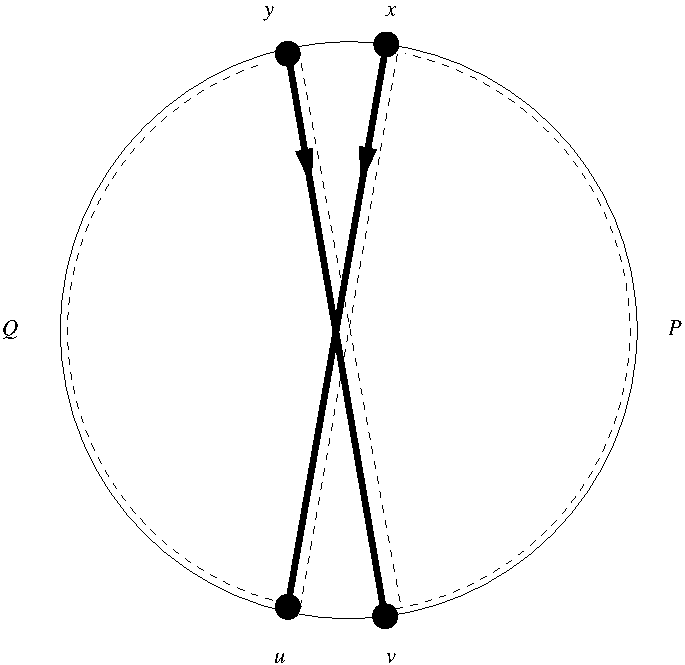
\includegraphics{forbid.pdf}} 
\caption[A forbidden configuration based on minimality]
{The Hamiltonian cycle $H$ is represented by a circle, and similarly $H'$ by a dashed line.  
The real arcs are represented by thicker lines.  \label{fig:forbid}} 
\end{figure} 
 

 \newpage
\subsection{Relay Vertices and Wedges}



For each virtual arc $(u,v)$ of $H$, we assign  
a real directed $uv$-path of length two.   
This assigned path is called the \emph{relay path} of the arc $(u,v)$.   
The fact that a relay path exists for every virtual arc follows from the definition of $\vec{G^2}$.   
The unique internal vertex of the relay path  
is called the \emph{relay vertex} of the arc $(u,v)$.  Note that more than one such real directed path may exist for  
a virtual arc.  The relay paths can be chosen arbitrarily, it is only important that they are fixed.   
   
 
 

A vertex may be the relay vertex for more than one 
virtual arc.  Hence we will group together %consecutive 
virtual arcs that are consecutive on $H$ if they have the same relay vertex.  
If $P$ is a maximal virtual (directed) 
path in $H$ containing more than one vertex, such that all virtual arcs of $P$ share a common relay vertex $w$,  
then the subgraph $W$ of $\vec{G^2}$ consisting of $P$, and the relay path of every arc of $P$, is  
called a \emph{wedge}; see Figure \ref{fig:wedge} for an example.  
We call $P$ the \emph{virtual path of the wedge} $W$.  
Similarly, arcs of $P$ are called \emph{virtual arcs of the wedge} $W$, and the vertex $w$ is called 
the \emph{relay vertex of the wedge} $W$.  Real arcs of  
$W$ are called  \emph{ribs} of $W$.  If we suppose the terminal vertices of $P$ are $u$ and $v$ such that 
$P$ is a $uv$-path, we refer to $u$ as the 
\emph{left external vertex} of $W$, and 
$v$ as the \emph{right external vertex} of $W$; both are called \emph{external vertices} of $W$.  Internal vertices  
of $P$ are called \emph{internal vertices} of the wedge.  The rib $(u,w)$  
is the \emph{left external rib} of $W$, and the rib  
$(w,v)$ is the \emph{right external rib} of the $W$; they are both referred to as \emph{external ribs} of $W$.  Real  
arcs of $W$ that are incident to an internal vertex are called \emph{internal ribs} of $W$.  %If $x$ is 
We define the \emph{size} of a wedge $W$, denoted $s(W)$, as the number of 
vertices of its virtual path.    
 
\begin{figure}[htp] 
\centering 
\resizebox{9cm}{!}{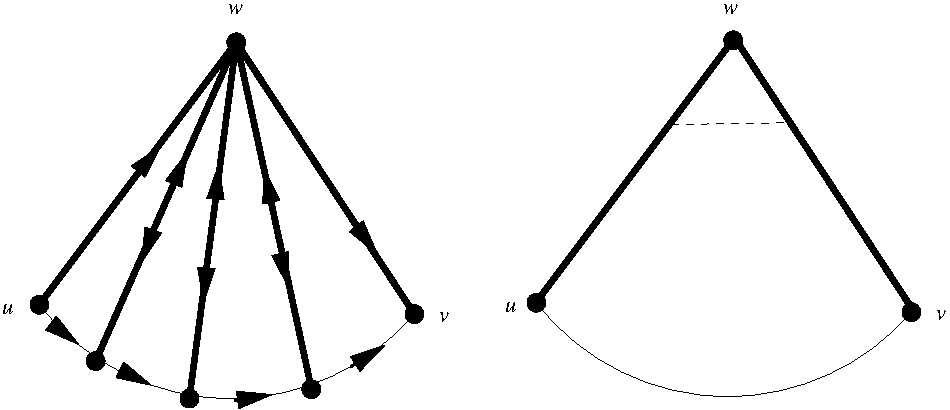
\includegraphics{wedge.pdf}}\\ 
\caption[A wedge of size five]{A wedge of size five.  The ribs are real arcs of $\vec{G^2}$ and are represented in this figure  
by thicker lines.  The virtual path consists of virtual arcs of $\vec{G^2}$ and are represented by regular lines.\label{fig:wedge}} 
\end{figure} 
 

Note that ribs of a wedge are always real arcs of $\vec{G^2}$.  
%However, an external 
%rib of a wedge may be incident to consecutive vertices of $H$.  
%Indeed, if $(w,v)$ is the right external rib of a wedge $W$ such that its inverse $(v,w)$ is an arc of $H$, 
%then the wedge $W$ is a \emph{right tied} wedge; similarly  
%if $(u,w)$ is the left external rib of $W$ such that $(w,u)$ is an arc of $H$, then the wedge is a \emph{left tied} wedge.  
%A wedge that is neither left tied nor right tied is called a \emph{free wedge}.   
The following lemma characterizes how two wedges can interact. 
 
\begin{lemma}\label{lemwedge} Suppose $W_1$ and $W_2$ are distinct wedges.  Then \newline 
$(i)$  The wedges $W_1$ and $W_2$ have no virtual arcs in common.  \newline 
$(ii)$  The wedges $W_1$ and $W_2$ have no ribs in common.\newline   
$(iii)$  If $e$ is a rib of $W_1$, $e^{-1}$ is not a rib of $W_2$.
\end{lemma} 
\begin{proof} 

Let $W_1$ and $W_2$ be wedges with relay vertices $w_1$, $w_2$ 
and virtual paths $P_1$, $P_2$, respectively.   

To show $(i)$, suppose to the contrary that $e$ is a virtual arc of both $W_1$ and $W_2$.   
Now $w_1$ is the relay vertex of $e$, since $e$ is a virtual arc of $W_1$.  But 
$e$ is also a virtual arc of $W_2$, so $w_2$ is the relay vertex of $e$.  Hence $w_1 = w_2$, since 
each virtual arc has exactly one relay vertex.  Now, since we 
supposed that $W_1 \ne W_2$, it follows that $P_1 \ne P_2$.  Since $e$ is an arc of both $P_1$ and $P_2$, it must be the case that  
either one of the paths is a subpath of the other, contradicting the maximality of the smaller path; or $P_1$ and $P_2$ overlap, in  
which case neither path is maximal, again a contradiction. 
Therefore $W_1$ and $W_2$ have no virtual arcs in common. 
 

%\begin{figure}[htp] 
%\centering 
%\resizebox{6cm}{!}{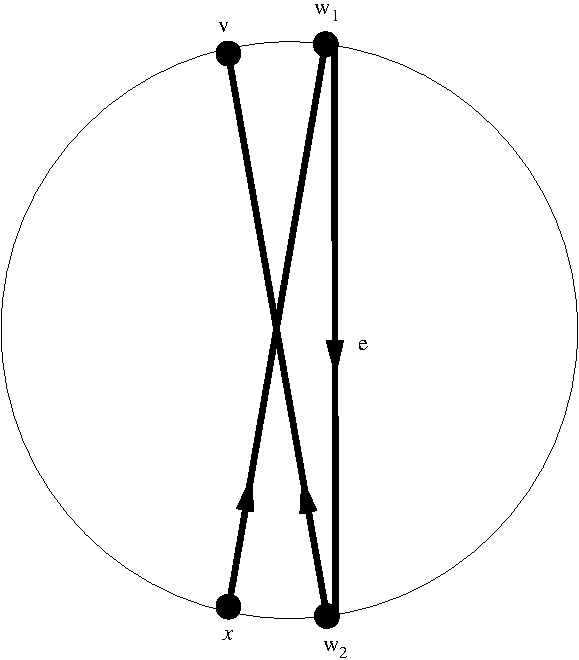
\includegraphics{fbw.pdf}} 
%\caption{insert generic caption \label{fig:fbw}} 
%\end{figure} 
 
We prove $(ii)$ in two cases, first suppose $w_1= w_2$.  Suppose 
to the contrary that $e$ is a rib of both  
$W_1$ and $W_2$.  If $e$ is an internal 
rib of either $W_1$ or $W_2$, then $v$ is incident to a virtual arc that is in both $P_1$ and $P_2$, which contradicts 
$(i)$.  
So $e$ is an external rib of both $W_1$ and $W_2$.   
Suppose that 
$e$ is the right external rib of $W_1$, (the case 
where $e$ is a left external vertex of $W_1$ is symmetric).  So $e=(w_1,v)$ such that $v$ is the right external vertex  
of $W_1$, (and $v\ne w_1$).  If $e$ is also the right external rib of $W_2$, then $v$ is incident to a virtual arc that is in both 
$P_1$ and $P_2$, which contradicts $(i)$.  Therefore $e$ is the left external rib of $W_2$.  Let $u$ be the left 
external vertex of $W_2$, so $e=(u,w_2)$ is the left external rib of $W_2$.  This is a contradiction, since the head 
of $e$ is $v=w_2=w_1$, and $v\ne w_1$.  


%Since $e$ is not an internal rib of $W_2$, $v$ is an external vertex of $W_2$.  If $v$ is also the right external vertex of 
%$W_2$, then $v$ is incident to a virtual arc that is in both wedges, which contradicts $(i)$.  
%So $v$ is the left external vertex of $W_2$, see Figure \ref{fig:wedgedub}.  
%This implies $e=(v,w_2)$.  Hence $e=(w_1,v)=(v,w_2)=(v,w_1)$, a contradiction since $v\ne w_1$.  


%Now suppose $w_1 \ne w_2$.  Suppose to the contrary the real arc $e$ of $\vec{G^2}$ is a 
%rib of both wedges.  This implies $e$ is incident to both relay vertices.  Without loss of generality, 
%let $e=(w_1,w_2)$, (the case when $e=(w_2,w_1)$ is similar).

%But $e$ cannot be the left  
%external rib of $W_2$, then the union of $P_1$ and $P_2$ is a longer path than both $P_1$ and $P_2$ alone, and all arcs  
%in the union are virtual and share the same relay vertex.  This contradicts the choice of $P_1$ and $P_2$, hence the  
%wedges have no ribs in common, so $(b)$ is proven. 

%suppose that $e$ is an arc common to both wedges.  From $(a)$, $e$ is not a virtual arc, so it must be a rib of  
%both wedges.  Also, from $(b)$ we know that $w_1 \ne w_2$.  Since $e$ is a rib of both $W_1$ and  
%$W_2$, this forces $e=w_1w_2$.  So  
%$w_1$ is also an internal vertex of $W_2$, and $w_2$ is also an internal vertex of $W_1$; see Figure \ref{fig:wedgeflip}. 
%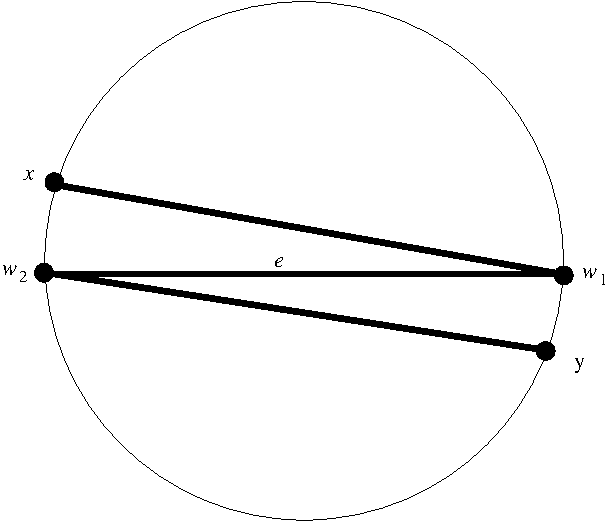
\includegraphics{wedgeflip.pdf} 

Now suppose $w_1 \ne w_2$.  Suppose to the contrary the real arc $e$ of $\vec{G^2}$ is a 
rib of both $W_1$ and $W_2$.  This implies $e$ is incident to both $w_1$ and $w_2$.  Without loss of generality, 
let $e=(w_1,w_2)$.  
First we will show that $w_1$ is an external vertex of $W_2$, and similarly $w_2$ is an external vertex of $W_1$.   
Suppose to the contrary 
that $w_1$ is an internal vertex of $W_2$, (we obtain a similar contradiction if 
$w_2$ is an internal vertex of $W_1$).  
Therefore there are two virtual arcs of $W_2$ incident with $w_1$, say $(u,w_1)$ and $(w_1,v)$.  
There is at least one virtual arc of $W_1$ incident with $w_2$, call it $h$.  
Suppose that $h=(x,w_2)$.  We know that $(x,w_1)$ is a real arc since  
it is a rib of $W_1$, similarly $(w_2,v)$ is a real arc since it is a rib of $W_2$, see Figure \ref{fig:fbw}.  
This contradicts Lemma \ref{obsx}.  If $h=(w_2,x)$ we get a similar  
contradiction.  Therefore $w_1$ is an external vertex of $W_2$, and similarly $w_2$ is an external vertex of $W_1$.  
 
It follows that $e$ is an external rib of both $W_1$ and $W_2$.  Since $w_1$ is the 
tail of $e$, $e$ is the right 
external rib of $W_1$, and similarly $e$ is also the left external rib of $W_2$.  %; see Figure \ref{fig:wedgecross}$(ii)$.  
Therefore $(w_1,v)$ is a virtual arc of the wedge $W_2$, and 
$(x,w_2)$ is a virtual arc of the wedge $W_1$, see Figure \ref{fig:fbw}.  So $(x,w_1)$ and $(w_2,v)$ are ribs 
of their respective wedges.  As above, since all ribs are real arcs, this contradicts Lemma \ref{obsx}.  
This concludes the proof of $(ii)$.   



To show $(iii)$, let $e=(u,v)$ be a rib of $W_1$.  Suppose to the contrary that $e^{-1}=(v,u)$ is a rib of $W_2$.  If 
$e$ is an internal rib of $W_1$, then $e^{-1}$ is also an internal rib of $W_1$, which contradicts part $(ii)$.  
So $e$ is an external rib of $W_1$; similarly $e^{-1}$ is an external rib of $W_2$.  
Suppose without loss of generality that 
$e$ is the right external rib of $W_1$, (the case $e$ is the left external rib of $W_1$ is symmetric).  So $u=w_1$, and $v$ is the 
right external vertex of $W_1$.  

\begin{figure}[htp] 
\centering 
\resizebox{6cm}{!}{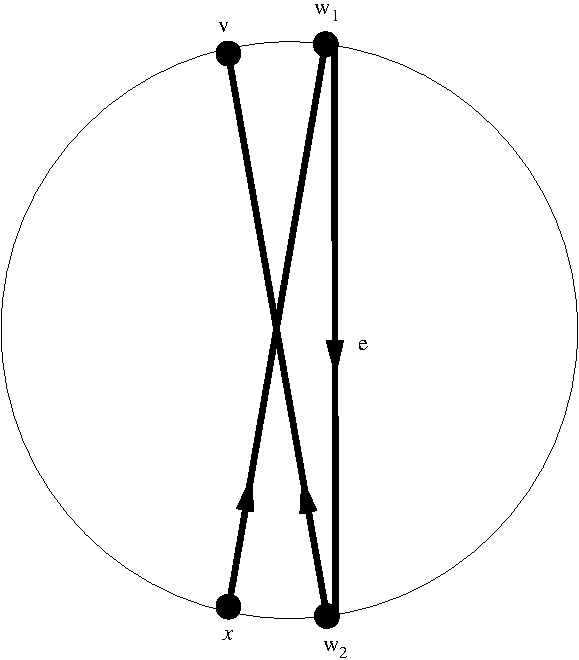
\includegraphics{fbw.pdf}} 
\caption[An edge in two relay paths]{The relay paths of the virtual arcs $(x,w_2)$ and $(w_1,v)$ both contain $e$.   \label{fig:fbw}} 
\end{figure} 
%\begin{figure}[htp] 
%\begin{minipage}[b]{0.5\linewidth}
%\centering 
%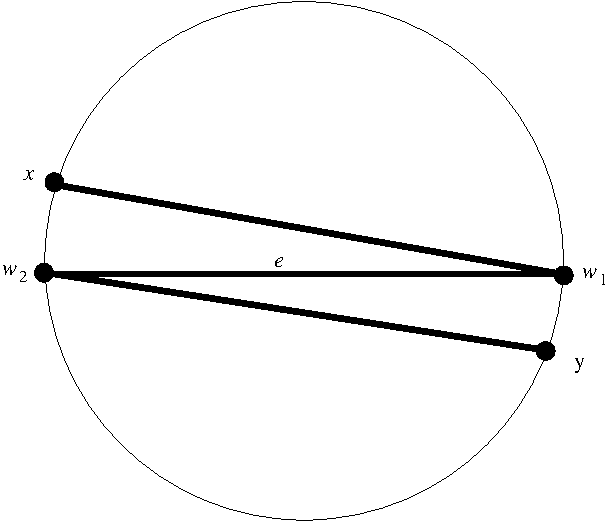
\includegraphics[width=6cm]{wedgeflip.pdf} 
%\newline
%$(i)$
%\end{minipage}
%\hspace{0.5cm}
%\begin{minipage}[b]{0.5\linewidth}
%\centering 
%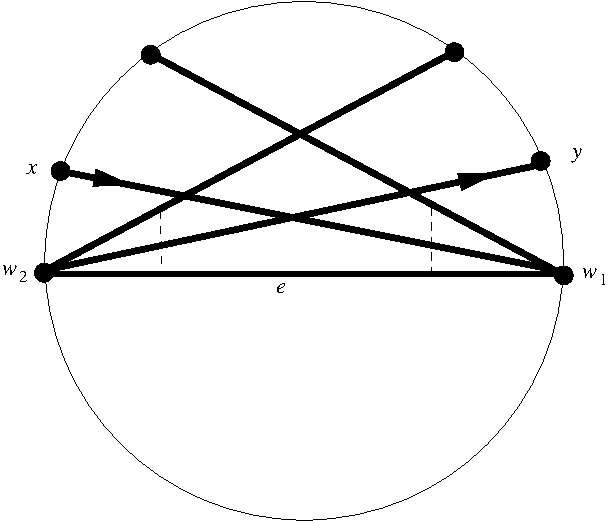
\includegraphics[width=6cm]{wedgecross.pdf}
%\newline
%$(ii)$
%\end{minipage}
%\caption{ The arcs $(y,w_1)$ and $(x,w_2)$ are virtual arcs of 
%$H$, and the edges $e$, $xw_1$ and $yw_2$, are real edges of $\vec{G}$. \label{fig:wedgecross}} 
%\end{figure} 


If $e^{-1}$ is 
the left external rib of $W_2$, then $u=w_2$ and $v$ is the left external vertex of $W_1$.    
So the union of $P_1$ and $P_2$ is a 
virtual path such that each (virtual) arc of this new 
path has relay vertex $u$, m
which contradicts the maximality of $P_1$ (and $P_2$).  

Next suppose $e^{-1}=(v,u)$ is the right external rib of $W_2$, and hence 
$v=w_2$.  Hence $e=(w_1,w_2)$, and $e^{-1}=(w_2,w_1)$.  Since $w_2$ is the right external vertex of the wedge $W_1$, there is a 
vertex $x$ such that $(x,w_2)$ is a virtual arc of $W_1$, and $(x,w_1)$ is a rib of $W_1$.  Similarly, there is a vertex $y$ 
such that $(y,w_1)$ is a virtual arc of $W_2$, and $(y,w_2)$ is a rib of $W_2$.  

Let $P$ be the path in $G$ containing 
the edges $xw_1$, $w_1w_2$, $w_2y$.  Since all these vertices are distinct, $P$ is a path of length three in $G$.  To show that $P$ is 
an induced subgraph of $G$, first notice that $xw_2$ and $yw_1$ are clearly virtual edges.  If $xy$ is a real edge, then $(x,y)$ and $(y,x)$ are 
real arcs, which contradicts Lemma \ref{obsx}.  So $xy$ is not a real edge, which implies $P$ is an induced subgraph of $G$, a contradiction 
since $G$ is $P_3$-free.  Therefore $e^{-1}$ is not a rib of $W_2$.  %This concludes the proof.   
\end{proof}


We can see that an external 
rib of a wedge cannot be an arc of $H$.  However, an external rib may be incident to consecutive vertices of $H$.  
Indeed, if $(w,v)$ is the right external rib of a wedge $W$ such that its inverse $(v,w)$ is an arc of $H$, 
then we say that the wedge $W$ is a \emph{right tied} wedge; similarly  
if $(u,w)$ is the left external rib of $W$ such that $(w,u)$ is an arc of $H$, then $W$ is a \emph{left tied} wedge.  
A wedge that is neither left tied nor right tied is called a \emph{free wedge}.   
Next, we show that there are not exist a  
wedge that is both left tied and right tied.  

\begin{lemma}\label{lemboth}
There does not exist a wedge of $\vec{G^2}$ that is both left tied and right tied.
\end{lemma}
\begin{proof}
Suppose to the contrary that the wedge $W$ is both left tied and right tied.  It is 
clear that $W$ contains all the vertices of $G$.  
Let $w$ be the relay vertex of $W$, $u$ be the left external vertex of $W$, and $v$ be the right external vertex of $W$.  
If $W$ contains only 
these three vertices, then $(u,v)$ is a virtual arc of $W$.  Hence there is no arc joining $u$ and $v$ 
in $\vec{G}$.  However, this implies that $w$ is a cut vertex in $G$, a 
contradiction since $G$ is $2$-connected.  Now suppose $G$ has at least four vertices.

\begin{figure}[htp] 
\centering 
\resizebox{6cm}{!}{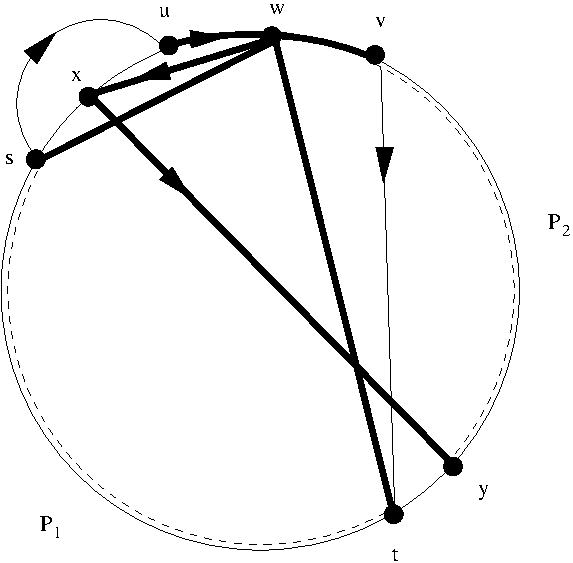
\includegraphics{bothtied.pdf}} 
\caption[Why a wedge cannot be both left and right tied]{The vertex $w$ is the relay vertex of a wedge that is both left tied and right tied.
\label{fig:bt}} 
\end{figure} 

Let $P$ be the virtual path of $W$, so $P$ is a directed $uv$-path.  Let $x\ne v$ be the vertex adjacent to 
$u$ on $P$.  Such a vertex exists since $\vec{G}$ has at least four vertices.  
Since $G$ is $2$-connected, $d(x) \ge 2$, so there is at least one real arc other than the ribs $(w,x)$ and $(x,w)$ incident to $x$, 
say $e=(x,y)$.  (Recall that we calculate the degree of a vertex with respect to $G$).  Since $(u,x)$ is a virtual arc, $u\ne y$, 
(but it is possible that $y=v$).  Since $(x,y)$ is a real arc, there exists at least 
one internal vertex of $W$ that lies between $x$ and $y$ on the path $P$; see Figure \ref{fig:bt}.  Let $s$ be the vertex 
following $x$ on $P$, and 
$t$ be the vertex preceding $y$ on $P$, (it is possible that $s=t$).  Let $P_1$ be the $st$-subpath of $P$, and $P_2$ be 
the $yv$-subpath of $P$, (either of which may not contain any arcs).  Since there is a real path of length two connecting $s$ and $u$, 
$(s,u)$ is either a real arc or a virtual arc of $\vec{G^2}$.  Similarly $(v,t)$ is an 
arc of $\vec{G^2}$, (that is either real or virtual).  

Let $H'$ be the cycle in $\vec{G^2}$ following 
$(u,w)$, $(w,x)$, $(x,y)$, $P_2$, $(v,t)$, $P_1^{-1}$, and $(s,u)$, see Figure \ref{fig:bt}.  
Clearly, $H'$ is a Hamiltonian cycle of $\vec{G^2}$.  
This is a contradiction since $H$ contains only two real arcs, (namely $(v,w)$ and $(w,u)$), while 
$H'$ contains at least three real arcs, (namely $(u,w)$, $(w,x)$, and $(x,y)$).  Therefore $W$ cannot be both left tied and right tied.
\end{proof}


For any vertex $v$, there may be several distinct wedges with relay vertex $v$; in the following we identify these wedges.  
If $v$ is the relay vertex of $k\ge 1$ wedges, we order these wedges at $v$ based on their occurrence along $H$.  
The \emph{list of ordered wedges} $W_1,W_2,\ldots,W_k$ \emph{at} $v$  
is the ordered list of all wedges with the common relay vertex $v$ such that for $W_i$ and $W_j$ with $i<j$, the virtual path of $W_i$  
occurs before the virtual path of $W_j$ when following $H$ starting from $v$; for example see Figure \ref{fig:wedgeorder}.  
When the list of ordered 
wedges at a vertex is understood, we will write $s_i$ for $s(W_i)$, (recall that $s(W)$ denotes the size of the wedge $W$).   
If $e$ is a  
real arc incident with $v$, we say that $e$ is an \emph{isolated arc} of $v$ if neither $e$ nor $e^{-1}$ are ribs of any wedge 
in the list of ordered wedges at $v$.


 
\begin{figure}[htp] 
\centering 
\resizebox{5cm}{!}{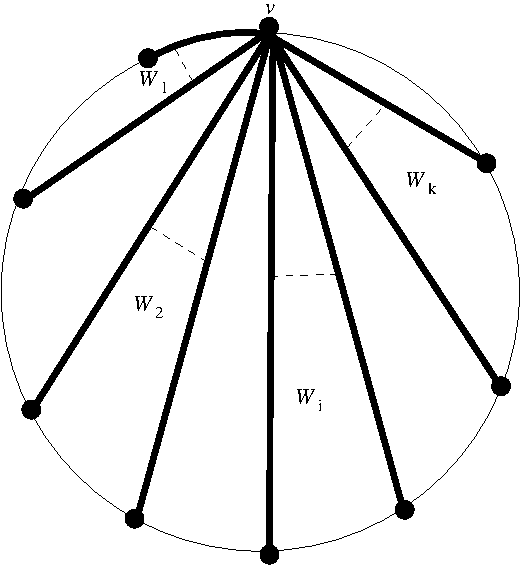
\includegraphics{wedgeorder.pdf}} 
\caption[The ordered list of wedges at a vertex]{The list of ordered wedges at $v$ is $W_1,W_2,\ldots,W_k$.  In this example, $W_1$ is a left tied wedge.  
\label{fig:wedgeorder}} 
\end{figure} 


In the Section \ref{sec:robot}, we will show how to turn the Hamiltonian cycle $H$ in $\vec{G^2}$ into a Hamiltonian walk $H^*$ in $\vec{G}$.  
To this end, we specify two arcs for each vertex, called the incoming and outgoing arcs of the vertex.  

\begin{definition}\label{def:io}
%If $e$ is a backtrack arc of $v$, then $e$ is an isolated arc of $v$.
Given a vertex $v$, let $(x,v)$ and $(v,y)$ be the two arcs of $H$ incident with $v$.  
\begin{itemize}
\item The incoming arc of $v$ is either   
$(x,v)$ if it is real, or the real arc $(w,v)$, where $w$ is the relay vertex of $(x,v)$.
\item Similarly, the  
outgoing arc of $v$ is either $(v,y)$ if it is real, or  
the real arc $(v,w)$, where $w$ is the relay vertex of $(v,y)$.  
\end{itemize}
If $e$ is the incoming arc of $v$ and 
$e^{-1}$ is the outgoing arc of $v$, we say that $e$ is a backtrack arc of $v$, (in which case 
$e^{-1}$ is also a backtrack arc of $v$).   
\end{definition}


Note that the incoming and outgoing  
arcs of a vertex are always real arcs.  By definition,  
each vertex has exactly one incoming arc, and one outgoing arc.  
Since the relay vertices of all virtual arcs are fixed, the incoming and 
outgoing arcs 
are also fixed for every vertex of $\vec{G}$.  In general, incoming and outgoing arcs of a vertex 
may or may not be isolated arcs of that vertex.  % (in Lemma \ref{lemmaext}, we further investigate the 
%cases where these arcs are not isolated).  
In the following we let $a$ and $b$ 
be the incoming and outgoing arcs of the vertex $v$, respectively

We first consider cases when $a\ne b^{-1}$, i.e., $v$ does not have a backtrack arc; there are four possible 
configurations.  If both $a$ and $b$ are 
real arcs of $H$, then they form a real path of length two along $H$ containing $v$ as an internal vertex, see Figure \ref{fig:iowedge}$(i)$.  
If $v$ is incident 
to two virtual arcs of $H$, then both $a$ and $b$ are arcs of disjoint relay paths, as shown in Figure \ref{fig:iowedge}$(ii)$.  Otherwise, 
exactly one of $a$ or $b$ is an arc of $H$, as shown in Figures 
\ref{fig:iowedge}$(iii)$ and \ref{fig:iowedge}$(iv)$.  
In the following lemma, we investigate how these arcs interact with wedges when they are not isolated arcs of $v$.  

\begin{figure}[htp] 
\centering 
\resizebox{9cm}{!}{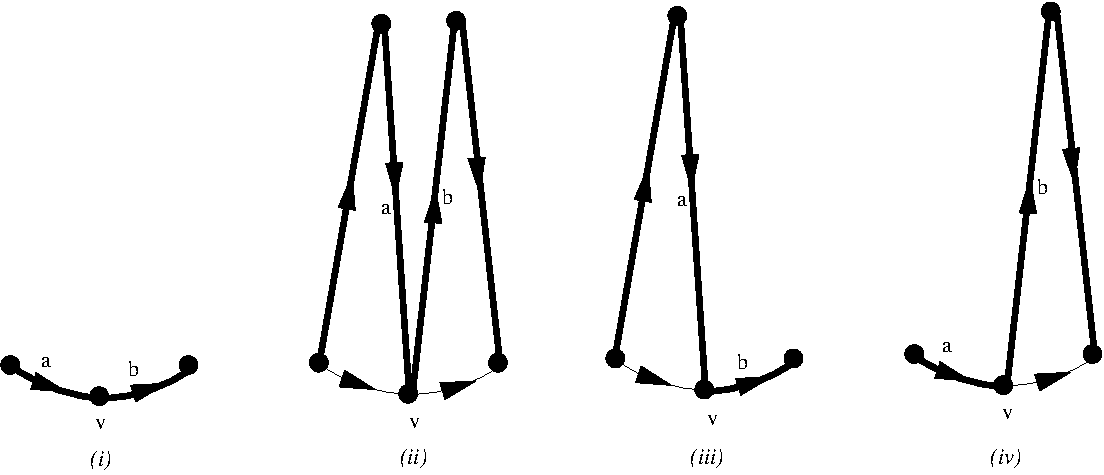
\includegraphics{iowedge.pdf}} 
\caption[The incoming and outgoing arcs of a vertex]
{The four of the possible configurations where $a$ is the incoming arc of $v$, $b$ is the outgoing arc of $v$, and $a\ne b^{-1}$.
\label{fig:iowedge}}
\end{figure} 
 


\begin{lemma}\label{lemmaext} 
Let $a$ be the 
incoming arc of $v$, and $b$ be the outgoing arc of $v$, such that $a\ne b^{-1}$.  Then:
 
\noindent $(i)$ If $a$ is not an isolated arc of $v$, then $a^{-1}$ is the right external 
rib of a right tied wedge $W$ with relay vertex $v$.

\noindent $(ii)$ If $b$ is not an isolated arc of $v$, then $b^{-1}$ is the left external 
rib of a left tied wedge $W$ relay vertex $v$.   %   
\end{lemma} 
\begin{proof} 

We prove only $(i)$; the proof for $(ii)$ is symmetric.  
Suppose $a$ is not an isolated arc of $v$.  It follows that either $a$ or $a^{-1}$ is a rib of some wedge with relay vertex $v$.  
First we show that $a=(u,v)$ cannot be a rib of any wedge with relay vertex $v$.  
%Then we will show that $a^{-1}$ must be a rib of a right tied wedge with relay vertex $v$.  % Finally, we will show that this wedge must be right tied.

To this end, suppose to the contrary that $a$ is 
a rib of the wedge $W$ with relay vertex $v$.  It follows that $a$ is not an arc of $H$, because 
wedges cannot contain any real arcs of $H$.  Hence, by Definition \ref{def:io}, $u$ 
is the relay vertex of the virtual arc $(x,v)$, (and $u\ne v$).  So $u$ is the relay vertex of some wedge $W'$ containing $(x,v)$.   
But now $a$ is a rib of both $W$ and $W'$.  Clearly $W\ne W'$, since 
they have different relay vertices.  This contradicts Lemma \ref{lemwedge}$(ii)$.  Therefore $a$ is not a rib of any wedge with 
relay vertex $v$.


Since $a$ is not an isolated arc of $v$, we conclude that there exists a wedge $W$ with relay vertex $v$ such that $a^{-1}$ is a rib of $W$.  
Since $a$ is the incoming arc of $v$, we have two cases by Definition \ref{def:io}.  
First, suppose that $a$ is an arc of $H$.  
Since $a=(u,v)$ is a real arc of $H$, it follows that $u$ is the right external vertex of the right tied wedge $W$.  
Thus $a^{-1}=(v,u)$ is 
the right external rib of $W$.  %Furthermore, since $(u,v)$ is an arc of $H$, $W$ is right tied.

For the second case, suppose $a$ is not an arc of $H$.  Hence $(x,v)$ is a virtual arc 
of $H$ such that $u$ is the relay vertex of $(x,v)$, (by Definition \ref{def:io}).  This implies there is a wedge $W'$ with 
relay vertex $u$ such that $(x,v)$ is a virtual arc of $W'$.  Hence $a$ is a rib of $W'$.  However, this 
contradicts Lemma \ref{lemwedge}$(iii)$, since $a^{-1}$ is a rib of $W$, and $W\ne W'$.   

\end{proof} 
 


In the following, we consider the case when $a=b^{-1}$.  The next lemma shows that in this situation, $a$ and $b$ 
must be isolated arcs of $v$.


\begin{lemma}\label{lemmaback} 
If $a$ is the incoming arc of $v$, and $b$ is the outgoing arc of $v$, and $a=b^{-1}$, then $a$ and $b$ are 
isolated arcs of $v$.
%If $e$ is a backtrack arc of $v$, then $e$ is an isolated arc of $v$.  
%For any vertex $v$, and real arc $e=(u,v)$, $e$ is a backtrack arc of $v$ if and only if  
%either $e$ is the internal rib of some wedge with relay vertex $w\ne v$;  
%or $e$ is both an arc of $H$ and an external rib of some tied wedge with relay vertex $w \ne v$, see Figure \ref{fig:wedgebkt}. 
\end{lemma} 
\begin{proof} 



\begin{figure}[htp] 
\begin{minipage}[b]{0.5\linewidth}
\centering 
{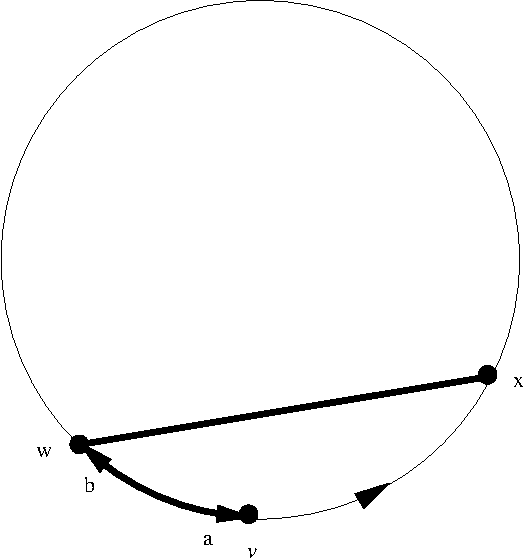
\includegraphics[width=6cm]{wedgebka.pdf}} 
\newline
$(i)$
\end{minipage}
\hspace{0.5cm}
\begin{minipage}[b]{0.5\linewidth}
\centering
{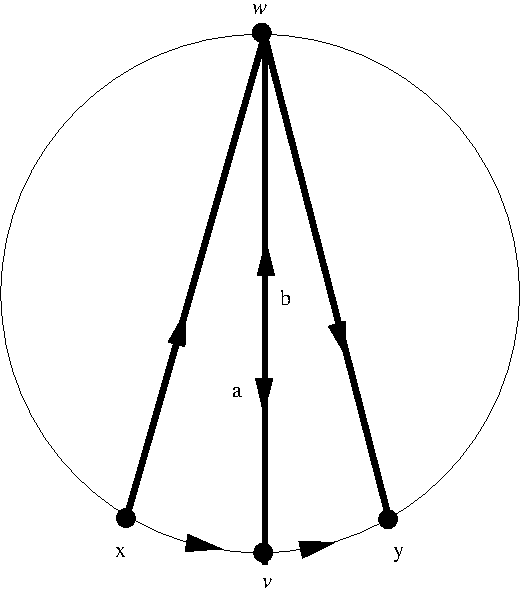
\includegraphics[width=6cm]{wedgebkb.pdf}} 
\newline
$(ii)$
\end{minipage}
\caption[Examples of a backtrack arc of a vertex]{Two of the three possible configurations showing backtrack arcs of $v$, 
where $a$ is the incoming arc of 
$v$ and $b$ is the outgoing arc of $v$, and $a=b^{-1}$.  \newline  
$(i)$  The vertex $v$ an external vertex of a tied wedge with relay vertex $w\ne v$.  \newline  
$(ii)$ The vertex $v$ is an internal vertex of a wedge with relay vertex $w\ne v$.  \label{fig:wedgebkt}} 
\end{figure} 


By Definition \ref{def:io}, there are two cases for each of $a$ and $b$, and hence four cases total.  First suppose both $a$ and $b$ are 
arcs of $H$.  Since $a=b^{-1}$, and since $H$ is a directed cycle, $H$ contains only these two arcs, and hence $H$ has two vertices.  
This is a contradiction since $\vec{G}$ has at least three vertices.  


Next suppose $a$ is an arc of $H$, and $b$ is not.  So $a$ is not a rib of any wedge.  By Definition \ref{def:io}, 
$b=(v,w)$ such that $w$ is the relay vertex of the virtual arc $(v,x)$ of $H$, see Figure \ref{fig:wedgebkt}$(i)$.  Now 
$w$ is the relay vertex for a left tied wedge $W$, and $b$ is the left external rib of $W$.  
By Lemma \ref{lemwedge}$(ii)$, $b$ is not a rib of any wedge with relay vertex $v$.  Therefore $a$ and $b$ are isolated arcs of $v$.  
If $b$ is an arc of $H$ and $a$ is not, the argument is similar.  

%Now 
%suppose to the contrary that $a$ is not an isolated arc of $v$, so $a$ is a rib of the wedge $W'$ with relay vertex $v$.  Since $a=(w,v)$ is 
%an arc of $H$, $a$ is the right external rib of $W'$, and $W'$ is a right tied wedge.  This contradicts Lemma \ref{lemwedge}$(iii)$, 
%since $b$ is the left external rib of $W$, and $a$ is the right external rib of $W'$, and $a=b^{-1}$.  Thus 
%$a$ and $b$ are isolated arcs of $v$.  
%If $b$ is an arc of $H$ and $a$ is not, we again obtain the desired result with a symmetric argument.  


Finally, suppose neither $a$ nor $b$ are arcs of $H$.  By Definition \ref{def:io}, $a=(w,v)$ such that $w$ is the relay vertex of the 
virtual arc $(x,v)$, and similarly $b=(v,w)$ such that $w$ is the relay vertex of the virtual arc $(v,y)$.  Hence $a$ and $b$ are 
internal ribs of the wedge $W$ with relay vertex $w$, see Figure \ref{fig:wedgebkt}$(ii)$.  
By Lemma \ref{lemwedge}$(ii)$, this implies neither $a$ nor $b$ are ribs of any wedge other than $W$.  Therefore, 
they are isolated arcs of $v$, (since $w\ne v$).  


\end{proof} 



We now have a good understanding of how wedges interact with these incoming and outgoing arcs.  
The next section describes how to assign port numbers to the arcs of $\vec{G}$.

\newpage
\subsection{Assigning Port Numbers}
\label{sec:pn}


In the previous section, we have defined wedges, and identified the incoming and outgoing arcs for every vertex.  
In this section, we will assign a label 
to each arc of $\vec{G}$, called a \emph{port number}.  
%These port numbers will be positive integers not greater than the degree of the vertex 
%plus three.  
Once assigned, these port numbers will be 
used by the robot in Section \ref{sec:robot} for the periodic traversal of $\vec{G}$.  


Let $e$ be an arc of $\vec{G}$.  One port number will be assigned to $e$, and one will be assigned 
to $e^{-1}$.   When every arc has a port, we call this a \emph{port numbering} of $\vec{G}$.  
If each arc has exactly one port number that is chosen uniquely from the set 
$\{ 1 , 2 , 3 , \ldots , d(v)\}$, where $v$ is the tail vertex of the arc, we call this a \emph{valid} port numbering of $\vec{G}$.  
%When every arc has a port, we call this a \emph{port numbering} of $\vec{G}$.  
When comparing two port numbers, we use 
the natural ordering of integers.  By associating these port numbers with the tail of the arc, this will induce 
a local orientation of the underlying graph $G$, (where each edge has two ports, one at each vertex).   
 
  
We will now describe how to assign an interval of port numbers to some ribs of a wedge.   
Given any wedge $W$ with relay vertex $v$,  
and virtual path $P=u_1,u_2,\ldots,u_{s(W)}$, we  
say that an interval $[p,q]$ \emph{is assigned to the wedge} $W$ if $1\le p<q \le d(v)$, $s(W)=q-p+1$, and 
port $p+i-1$ is assigned to $(v,u_i)$ for all $1\le i\le s(W)$.   
We say that the interval $[p,q]$ \emph{is assigned to} a set of wedges $\{W_1,W_2,\ldots,W_k\}=\{W_i\}_{i=1}^k$, 
if all wedges have a common relay vertex, 
$\sum_{i=1}^k s(W_i) = q-p+1$, 
$[p,p+s(W_1)-1]$ is assigned to $W_1$, and 
$[p+\sum_{i=1}^{j-1} s(W_i), p+\sum_{i=1}^j s(W_i) -1]$ is assigned to $W_j$ for $1< j\le k$.  

 
The assignment of the port numbers will be accomplished by applying the Port-Numbering procedure detailed below to 
each vertex $v$ of $\vec{G}$.  After identifying the incoming and outgoing arcs of $v$, there are five ways 
that these arcs can interact with wedges.  This leads to the five exclusive conditions for the 
what we will refer to as the five subroutines of the Port-Numbering procedure, starting at lines 
\ref{line:sr1}, \ref{line:sr2}, \ref{line:sr3}, \ref{line:sr4}, and \ref{line:sr5}, respectively.  Each subroutine 
will first assign port numbers to the incoming and outgoing arcs of $v$ if they are isolated, and then assigns 
an interval of ports to every wedge with relay vertex $v$.  The only wedges that are considered seperately by 
the Port-Numbering procedure are 
tied wedges.  The ports and intervals are chosen so that 
the incoming and outgoing arcs always have consecutive port numbers.  
Finally, the Port-Numbering procedure will run the arbitrary-ports subprocedure, which 
arbitrarily assigns 
a port to each arc with tail vertex $v$ 
that does not already have a port.  This procedure also ensures that the port $d(v)$ is not assigned to any arc with tail 
vertex $v$ by the arbitrary-ports subroutine.  




\begin{center}\begin{tabular*}{\textwidth}{c}\hline\end{tabular*}\end{center}
\noindent \textbf{procedure Port-Numbering}$(v)$
\begin{algorithmic}[1] 
\STATE{Let $a$ be the incoming arc of $v$} %\label{line:t1}
\STATE{Let $b$ be the outgoing arc of $v$}%\label{line:t2}
\STATE{Set $k$ such that $v$ is a relay vertex of $k$ distinct wedges} %\label{line:t3}
\IF{ $k > 0$} %\label{line:t4}
   \STATE{Let $\{W_i\}_{i=1}^k$ be the list of ordered wedges at $v$}% \label{line:t5}
\ENDIF %\label{line:t6}



\IF{$a=b^{-1}$} \label{line:sr1}
\STATE{Assign $d(v)$} to $b$ \label{line:backtrack}
\IF{$k>0$}
  \STATE{Assign $[d(v)-\sum_is_i,d(v)-1]$ to $\{W_i\}_{i=1}^k$}\label{line:fill1} %
  \ENDIF
\ENDIF



\IF{$a\ne b^{-1}$ and both $a$ and $b$ are isolated arcs of $v$}\label{line:sr2}
\STATE{Assign $d(v)-1$ to $a^{-1}$}\label{line:iso1}
\STATE{Assign $d(v)$ to $b$} \label{line:iso2}
\IF{$k>0$}
    \STATE{Assign $[d(v)-\sum_is_i-1,d(v)-2]$ to $\{W_i\}_{i=1}^k$}\label{line:fill2}
\ENDIF
\ENDIF




\IF{$a\ne b^{-1}$ and both $a$ and $b$ are not isolated arcs of $v$}\label{line:sr3}
    %\STATE{Assign  $[d(v)-s_{1}-s_{k}+1,d(v)-s_1]$ to $W_{1}$\label{line:bothin}}
    \STATE{Assign   $[d(v)-s_{1} +1 ,d(v)]$ to $W_{1}$\label{line:bothout}}
   \STATE{Assign  $[d(v)-s_{1}-s_{k}+1,d(v)-s_1]$ to $W_{k}$\label{line:bothin}}
    \IF{$k \ge 3$}
      \STATE{Assign $[ d(v)-\sum_is_i+1,d(v)-s_1-s_{k}]$ to $\{W_i\}_{1<i<k}$     \label{line:fill3}}
    \ENDIF
\ENDIF %end subroutine



\IF{$a\ne b^{-1}$, $a$ is an isolated arc of $v$ but $b$ is not}\label{line:sr4}
  \STATE{Assign $d(v)-s_1$ to $a^{-1}$\label{line:onlya}}
  \STATE{Assign $[d(v)-s_1+1,d(v)]$ to $W_1$\label{line:outtied}} 
   \IF{$k \ge 2$}
       \STATE{Assign $[d(v)-\sum_{i}s_i,d(v)-s_1-1]$ to $\{W_i\}_{i>1}$\label{line:fill4}}
   \ENDIF
\ENDIF%end subroutine




\IF{$a\ne b^{-1}$, $b$ is an isolated arc of $v$ but $a$ is not\label{line:sr5}}
  \STATE{Assign $[d(v)-s_k,d(v)-1]$ to $W_k$\label{line:intied}}
  \STATE{Assign $d(v)$ to $b$\label{line:onlyb}}
\IF{$k \ge 2$}
  \STATE{Assign  $[d(v)-\sum_{i}s_i,d(v)-s_k-1]$} to $\{W_i\}_{i<k}$\label{line:fill5}
\ENDIF 



 
\ENDIF % matches final case
\STATE arbitrary-ports$(v)$
\end{algorithmic} 
\begin{center}\begin{tabular*}{\textwidth}{c}\hline\end{tabular*}\end{center}


In the following lemma, we show that the Port-Numbering procedure will generate a valid port numbering of $\vec{G}$.  


\begin{lemma}
The procedure Port-Numbering will produce a valid port numbering of $\vec{G}$.
\end{lemma}
\begin{proof}
It is sufficient to show the following:
\newline
$(i)$ If a vertex $v$ sees port $p$, then  $1\le p\le d(v)$. \newline
$(ii)$ If two distinct arcs share the same tail vertex, they are assigned different ports.\newline
$(iii)$ Every arc of $\vec{G}$ has been assigned exactly one port. 


To show $(i)$, suppose that the arc $e=(v,u)$ has port $p$.  Let $a$ be the incoming arc of 
$v$, and $b$ be the outgoing arc of $v$.  

If $p$ was not assigned in an interval, then 
by inspection of the procedure, 
$p$ is either $d(v)-1$, $d(v)$, or $d(v)-s_1$.  Consider $p=d(v)-s_1$; the other cases are trivial.  So 
$p$ was assigned on line \ref{line:onlya}, which is part of the subroutine on line \ref{line:sr4}.  So 
$s_1$ is the size of the wedge $W_1$.  Since $b$ is an isolated arc of $v$, $2\le s_1\le d(v)-1$.  Therefore 
$1\le p \le d(v)$.

Now suppose $p$ belongs to 
some interval $I=[q,r]$, where $I$ was assigned to some wedge (or set of wedges) with relay vertex $v$.  
Let $W_1,W_2,\ldots,W_k$ be the list of ordered wedges at $v$.  Since $q\le p\le r$, it is sufficient to 
show that $q\ge 1$, and $r\le d(v)$.  

First, we show that $q\ge 1$.  
By inspection of the procedure, $q$ is of the form 
$d(v)-\sum_is_i$, $d(v)-\sum_is_i-1$, or $d(v)-\sum_is_i+1$, where the 
sum is over some subset of $\{W_i\}_{i=1}^k$.  Consider the case where $q=d(v)-\sum_is_i-1$ on line \ref{line:fill2}; 
the other 
cases are similar.  Since this interval was assigned in the subroutine 
starting on line \ref{line:sr2}, both $a$ and $b$ are isolated arcs of $v$.  So $\sum_i s_i \le d(v)-2$, 
which implies $d(v)-2-\sum_is_i \ge 0$, and hence $q\ge 1$.

Next we show $r\le d(v)$.  By inspection of the procedure, 
$r$ is either $d(v)$, $d(v)-1$, $d(v)-2$, $d(v)-s_1$, $d(v)-s_1-s_k$, or $d(v)-s_i-1$.   However, since the size of a wedge 
is always positive, this is trivial.  

In all cases, $1\le p \le d(v)$, so this proves $(i)$.

To show $(ii)$, let $e=(v,u)$ and $e' = (v,u')$ be two arcs such that $u\ne u'$.  
Suppose that $e$ was assigned port 
$p$, and $e'$ was assigned port $p'$, by the Port-Numbering procedure.  If either of $p$ or $p'$ were assigned by the arbitrary-ports 
subprocedure, we are done since by definition these ports were chosen uniquely.  
Otherwise, both $p$ and $p'$ were assigned in the same subroutine 
of the Port-Numbering procedure, (since at most one subroutine is executed for each vertex).  
Notice that if $p$ and $p'$ are both ports in the same interval, then we are done since $u\ne u'$, (see  the definition of how 
intervals of ports are assigned to wedges).  From now on, suppose $p$ and $P'$ are not both in the same assigned interval.  


%Suppose $p$ and $p'$ do not both belong 
%to any single interval that was assigned in the Port-Numbering procedure.  
The five subroutines are disjoint, hence we consider them individually.  It is sufficient to show, for 
each subroutine, that every pair of intervals assigned is disjoint, 
and no port assigned outside of an interval is contained in some assigned interval.  This will imply that $p\ne p'$.  

Consider first the subroutine on line \ref{line:sr1}.  There is at most one interval assigned, and by line \ref{line:fill1}, the 
largest port in that interval is $d(v)-1$.  The port $d(v)$ assigned on line \ref{line:backtrack} is not 
contained in this interval.  Hence $p\ne p'$ since at most one of $p$ or $p'$ is contained in the interval, by supposition.

Next consider the subroutine on line \ref{line:sr2}, so the ports $d(v)-1$ and $d(v)$ were assigned on lines 
\ref{line:iso1} and \ref{line:iso2}, respectively.  There is at most one interval assigned in this subroutine, and by 
line \ref{line:fill2} the largest port contained in this interval is $d(v)-2$.   
  
Now consider the  subroutine on line \ref{line:sr3}.  
There were at most three intervals assigned, namely $[d(v)-s_1+1,d(v)]$, $[d(v)-s_1-s_k+1,d(v)-s_1]$, and $[d(v)-\sum_{i}s_i+1,d(v)-s_1-s_k]$, by 
lines \ref{line:bothout}, \ref{line:bothin}, and  \ref{line:fill3}, respectively.  
Clearly these are disjoint since 
$d(v)-s_1-s_k<d(v)-s_1-s_k+1<d(v)-s_1<d(v)-s_1+1$.   

The subroutine on line \ref{line:sr4} assigns port $d(v)-s_1$ on line \ref{line:onlya}, and it assigns at most two intervals.  
By lines \ref{line:outtied} and \ref{line:fill4}, we can clearly see that these intervals are disjoint and do not contain the port $d(v)-s_1$, 
since $d(v)-s_1-1<d(v)-s_1<d(v)-s_1+1$.

Finally, consider the subroutine on line \ref{line:sr5}.  So port $d(v)$ was assigned on line \ref{line:onlyb}.  There are 
at most two intervals assigned on lines \ref{line:intied} and \ref{line:fill5}.  These intervals clearly do not 
contain $d(v)$, and they are disjoint since $d(v)-s_k+1<d(v)-s_k$.  



Hence all cases, $p\ne p'$, so this proves $(ii)$.

To show $(iii)$, let $e=(v,u)$ be an arc of $\vec{G}$.  The Port-Numbering procedure will be executed at $v$ exactly once.  Hence the 
arc $e$ will be assigned a port by at most one of the five subroutines, 
(starting on lines \ref{line:sr1}, \ref{line:sr2}, \ref{line:sr3}, \ref{line:sr4}, and \ref{line:sr5}).  %The 
%conditions that invoke the subroutines are all exclusive, hence $e$ was considered by exactly one of them.  

If $e$ is not assigned a port in any of these five subroutines, then by definition that the 
arbitrary-ports subprocedure will always assign a port to $e$.  So $e$ always has at least one port number.


It remains to show that each subroutine assigns at most one port to $e$, (since they are exclusive).   
If 
$e$ was assigned a port outside of an interval, then $e$ is an isolated arc of $v$.  
We know $e$ belongs to at most one wedge by Lemma \ref{lemwedge}$(ii)$.  It is 
easy to verify in every case that the length of each interval is equal to the size of the corresponding wedge (or wedges) that the interval 
was assigned to.  For example, the length of the interval on line \ref{line:fill1} is $d(v)-1 -(d(v) - \sum_i s_i) +1 = \sum_i s_i$.  

Finally, we show that each wedge is assigned at most one interval.  The only case where this may not be clear is in the subroutine 
on line \ref{line:sr3}.  
Let $a$ be the incoming arc of $v$, $b$ be the 
outgoing arc of $v$, and let $W_1,W_2,\ldots,W_k$ be the list of ordered wedges at 
$v$.  %Recall that only $W_1$ and $W_k$ can be tied wedges.  
By Lemma \ref{lemmaext}, $a^{-1}$ is a rib of the tied wedge $W_1$ and $b^{-1}$ is a rib of the tied wedge $W_k$.  
We also know by Lemma \ref{lemboth} that $W_1$ is not right tied and $W_k$ is not left tied, so $k\ne 1$.    Therefore each wedge is 
assigned at most one interval.   and $e$ has exactly one port number.  

\end{proof}


Now we know that the Port-Numbering procedure is well defined, and it produces a valid port numbering of the graph $\vec{G}$.  In the next section, 
we define a robot that will perform the traversal of $\vec{G}$ by using these ports.  


\newpage
\subsection{The Invariant}

Now we define an invariant which will guarantee, under certain conditions, that the robot will periodically traverse $\vec{G}$.  
Let $H^*$ be the directed graph constructed by starting from $H$, then replacing every virtual arc of $H$ with its 
corresponding relay path.  Naturally, $H^*$ induces a (directed) Hamiltonian walk of $\vec{G}$ by 
following $H$, where each virtual arc is traversed via the corresponding relay path.  
Hence $H^*$ is a subgraph of $\vec{G}$.  We will abuse 
notation and identify the directed graph $H^*$ with this Hamiltonian walk of $\vec{G}$, and denote both by $H^*$.  When 
we refer to a port number of an arc of $H^*$, we of course mean the port number of the corresponding arc of the graph $\vec{G}$.  
Observe that if $W$ is a wedge, then every 
rib of $W$ is in $H^*$.  This implies that the incoming and outgoing arcs of a vertex are always in $H^*$.  

The fact that $H^*$ is a Hamiltonian walk gives rise to the natural successor function defined 
on arcs of $H^*$; the \emph{successor} of an arc $e$ of $H^*$ is the arc following $e$ on $H^*$, denoted by $e^+$.  
In particular, if $e$ is the incoming arc of $v$, then $e^+$ is the outgoing arc of $v$, see for example Figure \ref{fig:iowedge}.  
With this in mind, we define an invariant which will 
guarantee, under certain conditions, that the robot will periodically traverse $\vec{G}$. \\

\noindent \textbf{The Invariant:} \emph{If the robot enters a vertex on an arc $e$ of $H^*$, 
then the robot will leave that vertex on the arc $e^+$ of $H^*$.  }\\

The invariant guarantees a periodic traversal once the 
robot uses an arc of $H^*$ to enter a vertex.  The fact that 
the invariant always holds follows from Lemma \ref{lemmainvariant}.  First, we first prove that, given 
the correct initial configuration with any initial vertex, the robot always 
leaves the vertex on an arc of $H^*$, and hence enters the new current vertex on an arc of $H^*$.  

\begin{figure}[htp] 
\begin{minipage}[b]{0.5\linewidth}
\centering 
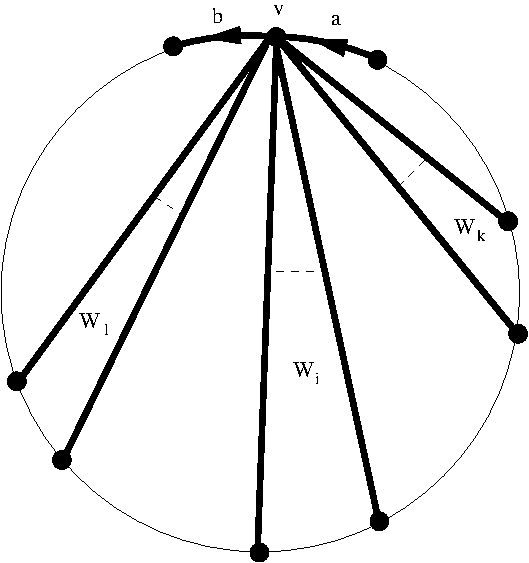
\includegraphics[width=6cm]{bothisoh.pdf}
\newline
$(i)$
\end{minipage}
\hspace{0.5cm}
\begin{minipage}[b]{0.5\linewidth}
\centering
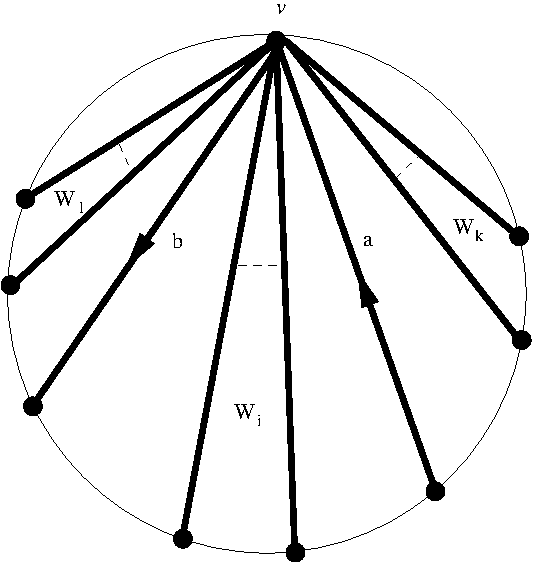
\includegraphics[width=6cm]{bothiso.pdf}
\newline
$(ii)$
\end{minipage}
\caption[The incoming and outgoing arcs of a vertex are both isolated]{Both $a$ and $b$ are isolated arcs of $v$.  Represented are two 
of the four possible configurations, depending on whether or not $a$ or $b$ are arcs of $H$.
In $(i)$ we depict the case where both $a$ and $b$ are arcs of $H$; in $(ii)$ we depict the case 
where neither $a$ nor $b$ are arcs of $H$. \label{fig:bothiso}}
\end{figure}



\begin{lemma}\label{lemmastart}
Let $v$ be any vertex of $G$.  Suppose the robot starts on the configuration $(d(v),v,\alpha)$.  
Then the robot will leave $v$ on an arc $e$ of $H^*$.  Hence if $e=(v,u)$, the robot will enter 
$u$ on an arc of $H^*$.
\end{lemma}
\begin{proof}  

%Suppose that the robot is placed at the initial vertex $v$.    
Let $a$ be the incoming arc of $v$, $b$ be the 
outgoing arc of $v$, and suppose that $v$ is the relay vertex of $k\ge 0$ distinct wedges.  
%Only case $(1)$ of the transition function can be applied here, since the robot will be in the initial state $\alpha$.  
Since the configuration of the robot has the entering port $d(v)$, the second case of the transition function will be applied.  Hence it is sufficient 
to show that the Port-Numbering procedure has assigned port $d(v)$ to an arc with tail vertex $v$, that is an arc of $H^*$.  
Recall that $H^*$ contains both $a$ and $b$, as well as 
any arc that is a rib of any wedge.  
There are five cases based on the subroutines of the Port-Numbering procedure. 



\noindent\textbf{Case 1: } Suppose first that $a=b^{-1}$.    
So the subroutine on line \ref{line:sr1} 
was executed $v$.  Port $d(v)$ was assigned to $b$ by line 
\ref{line:backtrack}, which is an arc of $H^*$.  

From now on, suppose $a\ne b^{-1}$.

\noindent\textbf{Case 2: } Suppose that both $a$ and $b$ are isolated arcs of $v$; for example 
see Figure \ref{fig:bothiso}.  
So the subroutine on line \ref{line:sr2} was executed at $v$.  So 
$b$ has port $d(v)$ by line \ref{line:iso2}.  


\noindent\textbf{Case 3: } Now suppose neither $a$ nor $b$ are isolated arcs of $v$; 
see Figure \ref{fig:noneiso}.  So the subroutine at line \ref{line:sr3} was executed at $v$.    
By line \ref{line:bothout}, the right external rib of $W_1$, (which is an arc of $H^*$), has port $d(v)$.  
 

\noindent\textbf{Case 4: } Now suppose $b$ is not an isolated arc of $v$, and $a$ is an isolated arc of $v$, for 
the two possible cases see Figure \ref{fig:onlyai}.  
So the subroutine at line \ref{line:sr4} was executed at $v$.    
Hence the right external rib of $W_1$, (which is an arc of $H^*$), was assigned port $d(v)$ by line \ref{line:outtied}.  


\noindent\textbf{Case 5: } Finally suppose $a$ is not an isolated arc of $v$, and $b$ is an isolated arc of $v$, 
so the subroutine at line \ref{line:sr5} was executed at $v$.  For the two possible cases see Figure \ref{fig:onlybi}.
By line \ref{line:onlyb}, $b$ has port $d(v)$.

\end{proof}

\begin{figure}[htp] 
\begin{minipage}[b]{0.5\linewidth}
\centering 
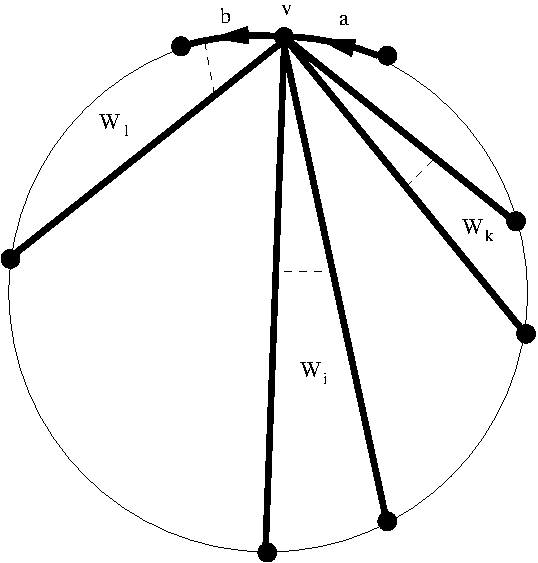
\includegraphics[width=6cm]{onlyaisoh.pdf}
\newline
$(i)$
%\caption{Non isolated arcs with a tied wedge\label{fig:athbr}} 
\end{minipage}
\hspace{0.5cm}
\begin{minipage}[b]{0.5\linewidth}
\centering
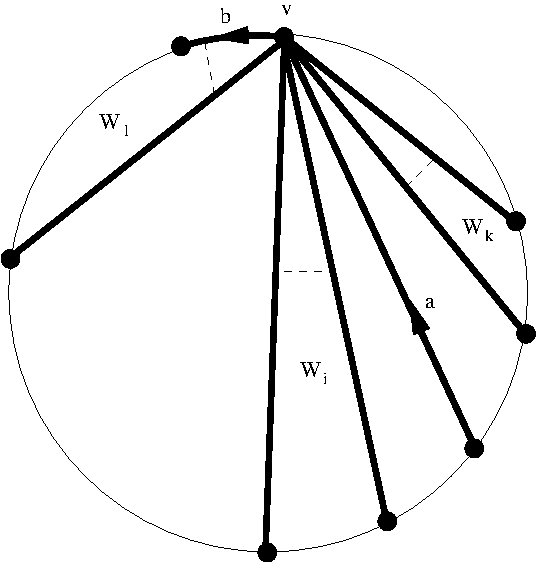
\includegraphics[width=6cm]{onlyaiso.pdf}
\newline
$(ii)$
%\caption{Non isolated arcs without a tied wedge}
\end{minipage}
\caption[The incoming arc of a vertex is isolated]{The arc $a$ is an isolated arc of $v$, and $b$ is not.  In $(i)$, $a$ is an 
arc of $H$, and in $(ii)$ it is not.  \label{fig:onlyai}}
\end{figure}



Now we know that at the initial step, the robot always enters the new current vertex along an arc of $H^*$.  
The following lemma implies that the invariant always holds, provided that the robot entered a vertex $v$ on an arc of 
$H^*$.  


\begin{lemma}\label{lemmainvariant}
Suppose the current configuration of the robot is $(p,v,\alpha)$, such that $v$ was entered on 
an arc $e$ of $H^*$.  Then the robot will leave on $e^+$, (which is an arc of $H^*$).  
%Let $v$ be the current vertex of the robot, $\alpha$ be the current state of the robot, and suppose 
%the robot entered $v$ along the arc $e$ of $H^*$.  Then 
%the robot will leave $v$ on $e^+$.
\end{lemma}
\begin{proof}

Let $e=(u,v)$, hence $p$ is the port number of $e^{-1}=(v,u)$.  
Suppose $T(p,v,\alpha)=(q,v',\alpha)$, so the robot leaves $v$ on the arc $(v,v')$, and the port of $(v',v)$ is $q$.  
It is sufficient to show that $e^+=(v,v')$.  


%, such that its 
%reverse $(v',v)$ has port $q$.
%Hence 
%it is sufficient to show that the arc $e^+=(v,v')$ has port $q$ such that $T(p,v,\alpha)=(q,v',\alpha)$.  
%Since the vertex $v'$ is implied whenever 
%the arc $e^+$ is defined, and since the robot will never leave state $\alpha$, we will abuse notation and write 
%$T(p,e)=(q,e^+)$ to represent $T(p,v,\alpha)=(q,v',\alpha)$.


Let $a$ be the incoming arc of $v$, $b$ be the outgoing arc of $v$, and $v$ 
be the relay vertex of $k\ge 0$ wedges.  First notice that, since the tail of $b$ is $v$, 
$e\ne b$, and similarly $e$ is not the right external rib of any wedge 
with relay vertex $v$.  Since $e$ is an arc of $H^*$, either $e=a$, or $e$ is an internal rib, or the left external rib of some wedge with 
relay vertex $v$.%, (indeed, if $e$ is either an arc of $H$ or a rib of some wedge with relay vertex $u$, then $e=a$).  

%The proof is laid out in five cases, each of which considers one subroutine 
%of the Port-Numbering procedure, and examines all the possible values of $p$.

In what follows, we will examine all possible values for the port $p$.  This will 
be done with respect to each of the five subroutines of the Port-Numbering procedure, (since the 
subroutines are exclusive, and we know $p$ was assigned in one of these subroutines since $e$ is an arc of $H^*$).  

\begin{figure}[htp] 
\centering
\resizebox{6cm}{!}{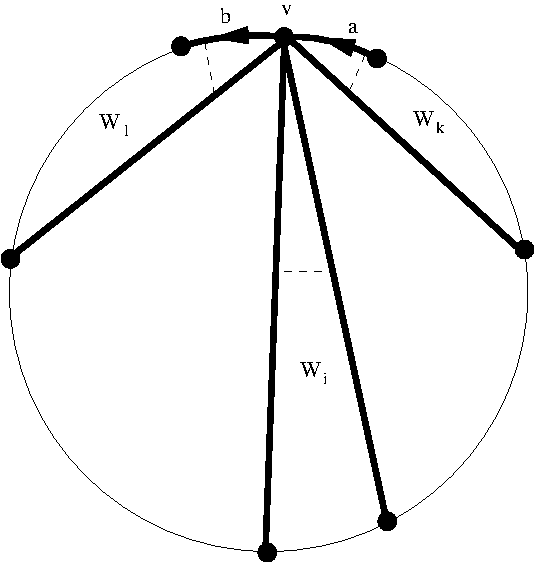
\includegraphics{noneiso.pdf}}
\caption[Neither the incoming nor outgoing arcs of a vertex are isolated]{Neither $a$ nor $b$ are isolated arcs of $v$.\label{fig:noneiso}}
\end{figure}



\noindent\textbf{Case 1: } Suppose first that $a=b^{-1}$; see Figure \ref{fig:wedgebkt}.  
So the subroutine on line \ref{line:sr1} was executed at $v$.  
By line \ref{line:backtrack}, the port of $a^{-1}=b$ is $d(v)$.  Hence if $p=d(v)$, then $e=a$, which implies 
$e^+=b$.  
Since the port of $e^+$ is $d(v)$, $e^+=(v,v')$.  
%v),e)=(d(v),e^+)$, (so the robot will leave $v$ on $e^+$).  %So the robot will leave $v$ on $e^+$.  

Now let $p< d(v)$.  %This implies, from line \ref{line:fill0}, that 
Since the port of $a^{-1}$ is $d(v)$, $e\ne a$.  Since $e$ is an arc of $H^*$, and $e\ne a$, it follows that 
$e$ is a rib of some wedge with relay 
vertex $v$, and hence $k>0$.  Let $W_1,W_2,\ldots,W_k$ be the list of ordered wedges at 
$v$.  So $e$ is a rib $W_j$ for some $1\le j\le k$.  %By line line \ref{line:fill1}, $p\le d(v)-1$.  
Furthermore, since $e$ is not 
the right external rib of $W_j$, there is a virtual arc 
$(u,x)$ of $W_j$ such that $e^+=(v,x)$ is a rib of $W_j$.  Clearly, $e^+$ was assigned port $p+1$ at $v$ by line \ref{line:fill1}.  
Since $p< d(v)$, $x=v'$ and hence $e^+=(v,v')$.

From now on, suppose $a\ne b^{-1}$.  

\begin{figure}[htp] 
\begin{minipage}[b]{0.5\linewidth}
\centering 
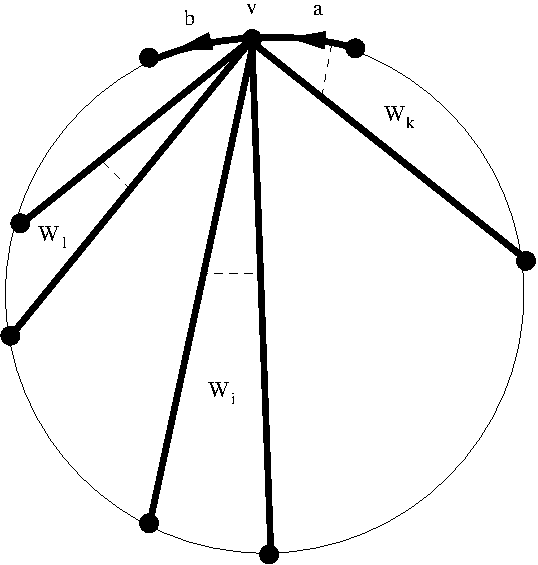
\includegraphics[width=6cm]{onlybisoh.pdf}
\newline
$(i)$
%\caption{Non isolated arcs with a tied wedge\label{fig:athbr}} 
\end{minipage}
\hspace{0.5cm}
\begin{minipage}[b]{0.5\linewidth}
\centering
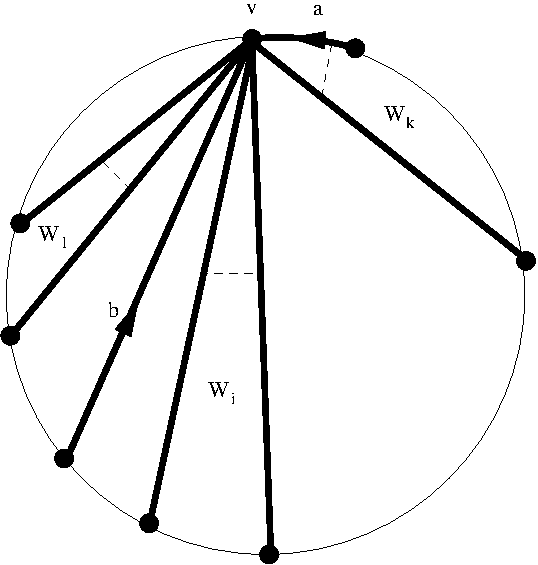
\includegraphics[width=6cm]{onlybiso.pdf}
\newline
$(ii)$
%\caption{Non isolated arcs without a tied wedge}
\end{minipage}
\caption[The outgoing arc of a vertex is isolated]{The arc $b$ is an isolated arc of $v$, and $a$ is not.  In figure $(i)$, $b$ is an 
arc of $H$, and in figure $(ii)$ it is not.  \label{fig:onlybi}}
\end{figure}




\noindent\textbf{Case 2: } Suppose both $a$ and $b$ are isolated arcs of $v$, see Figure \ref{fig:bothiso}.  
So the subroutine on line \ref{line:sr2} was executed at $v$.  
If $p=d(v)-1$, then $e=a$ by line \ref{line:iso1}, which implies $e^+=b$.  
Since $b$ has port $d(v)$ by line \ref{line:iso2}, $e^+=(v,v')$. %the robot will leave $v$ on $e^+$ by the transition function.  


Now let $p\ne d(v)-1$.  This implies $e\ne a$, and hence 
$e$ is a rib of some wedge with relay vertex $v$, which means $k>0$.    
Let $W_1,W_2,\ldots,W_k$ be 
the list of ordered wedges at $v$.  Let $e$ is a rib of $W_j$ for some $1\le j\le k$. 
Since the head of $e$ is $v$, $e$ is either an internal rib or the left external rib of $W_j$.  
So $e^+ = (v,x)$ where $(u,x)$ is a 
virtual arc of $W_j$.   
We know by by line \ref{line:fill2} that $e^+$ has port $p+1$, and $p<d(v)$.  Therefore $x=v'$, so $e^+=(v,v')$.
%the robot will leave $v$ on $e^+$ by the transition function.  

  
\noindent\textbf{Case 3: } Suppose that neither $a$ nor $b$ are isolated arcs of $v$, see Figure \ref{fig:noneiso}.  This implies 
that the subroutine on line \ref{line:sr3} was executed at $v$.  This also implies that $k\ge 1$, so let 
$W_1,W_2,\ldots,W_k$ be the list of ordered wedges at $v$.  
Hence, by Lemma \ref{lemmaext}, $a^{-1}$ is the right external rib of $W_j$, 
and $b^{-1}$ is the left external rib of $W_{j'}$, for $1\le j,j' \le k$.  Furthermore, since $W_j$ is right tied and 
$W_{j'}$ is right tied, $j=k$ and $j'=1$.  
Hence $b$ has port $d(v)-s_1+1$, and $a^{-1}$ has port $d(v)-s_1$, 
by lines \ref{line:bothout} and \ref{line:bothin}, respectively.  %Notice 
%that $p \le s_j < d(v)$, so only the transition function is applicable.  

Suppose $p=d(v)-s_1$, so $e=a$ and $e^+=b$.  
Since $e^+$ has port $p+1=d(v)-s_1+1$, and since $p<d(v)$, $e^+=(v,v')$. 

Next suppose $p\ne d(v)-s_1$, which implies $e\ne a$.  Thus $e$ is either an 
internal rib or the left external rib of some wedge $W_j$ for $1\le j\le k$.  Thus $v$ is the relay vertex of a virtual arc $(u,x)$ of $W_j$, such 
that $e^+=(v,x)$.  So port $p+1$ was assigned to $e^+$ (by either line  \ref{line:bothout}, \ref{line:bothin}, or \ref{line:fill3}).  
Therefore $x=v'$, hence $e^+=(v,v')$.   


\noindent\textbf{Case 4: } Next, we suppose that $b$ is not an isolated arc of $v$, and $a$ is an isolated arc 
of $v$, see Figure \ref{fig:onlyai}.  %, for example see Figure \ref{fig:onlyai}.    
So the subroutine at line \ref{line:sr4} was executed at $v$.  Since $b$ is not an isolated arc of $v$, we have $k>0$, 
so let $W_1,W_2,\ldots, W_k$ be 
the list of ordered wedges at $v$.  By Lemma \ref{lemmaext}, $b^{-1}$ is the left external rib of $W_j$ for some $1\le j\le k$.  Since 
$W_j$ is a left 
tied wedge, $j=1$.    

If $p=d(v)-s_1$, then $e=a$, which implies 
$e^+ = b$.  By line \ref{line:outtied}, $e^+$ has port $d(v)-s_j+1=p+1$, so $e^+=(v,v')$.  
%by the transition function, the robot will leave $v$ on $e^+$.  

Otherwise $p\ne d(v)-s_1$, so $e\ne a$.  Hence $e$ is a rib of some wedge $W_j$ with relay vertex $v$, where $1\le j\le k$.  
Since $e$ is not the right external rib of $W_j$, we have $p<d(v)$. 
As above, $e^+$ is a rib of $W_{j}$ such that $e^+$ has port $p+1$, either by line \ref{line:outtied} 
or \ref{line:fill4}.    
Therefore $e^+=(v,v')$.  
%by the transition function, 
%the robot will leave $v$ on $e^+$.

\noindent\textbf{Case 5: } Now suppose that $b$ is an isolated arc of $v$ and $a$ is not, see Figure \ref{fig:onlybi}.  So 
the subroutine on line \ref{line:sr5} was executed at $v$.  
Since $a$ is not an isolated arc of $v$, $k>0$, so let $W_1,W_2,\ldots,W_k$ be the list of ordered wedges at $v$.  By 
Lemma \ref{lemmaext}, 
$a^{-1}$ is the right external rib of $W_k$.  By line \ref{line:intied}, $a^{-1}$ has 
port $d(v)-1$.  

If $p=d(v)-1$, then $e=a$, which 
implies $e^+ =b$.  Since $e^+$ has port $p+1=d(v)$ by line \ref{line:onlyb}, $e^+=(v,v')$. 
%by the transition function the robot will leave $v$ on $e^+$.  

Now suppose $p\ne d(v)-1$.  
So $e$ is either an internal rib, or the left external rib of $W_j$, for some $1\le j\le k$.  As in previous cases, 
$e^+$ is the rib of $W_j$ that has port $p+1$ by either line \ref{line:intied} or \ref{line:fill5}, 
(and it is clear that $p<d(v)$).  Thus $e^+=(v,v')$. 
%the robot will leave $v$ on $e^+$ by the transition function.



 
In all five cases, the robot left $v$ on the arc $e^+$ according to the transition function.  
The proof of the invariant follows.





\end{proof}

\newpage
\section{Upper Bound of the Period} \label{umain}

 We obtain an upper bound on the period of this traversal.  
 


\begin{theorem}\label{pmain}
Let $G$ be a $P_3$-free graph, with $\delta(G)\ge 2$.  Then there exists a local orientation of $G$ and a corresponding 
robot (defined in Section \ref{sec:robot}) that 
will perform a periodic traversal of $G$ with period $\pi (n) \le 2n-2$, (provided the robot starts in configuration $(d(v),v,\alpha)$, 
where $v$ is any vertex of $G$).
\end{theorem} 
\begin{proof} 
 
If $G$ is not $2$-connected, then by Lemma \ref{lemclass}, $\Delta(G)=n-1$.  Hence we will fix the local orientation of $G$ using 
the Star-Numbering procedure.  By Lemma \ref{lemstar}, every vertex of $G$ is visited periodically, with period at most $2n-3$.  


Now suppose $G$ is $2$-connected.  
The result of Fleishner from \cite{FL} guarantees that $H$ exists.  Suppose $H^*$, the robot, and the ports of $G$ 
are as described above.  
By Lemma \ref{lemmastart}, the robot will leave $v$ on an arc of $H^*$.  After this step, by 
Lemma \ref{lemmainvariant}, the robot will start periodically traversing arcs of $H^*$, and hence every vertex of $G$.  

Next we estimate 
the period of the traversal, $\pi(n)$.  
Recall that the period $\pi(n)$ of the traversal 
is the maximum number of arcs traversed between two consecutive visits of any vertex.  


For any arc $e=(u,v)$ of $H$, the robot will traverse at most two arcs to get from $u$ to $v$; one if $e$ 
is real and two if $e$ is virtual.  

The maximum number of arc traversals between two visits of $v$ will clearly occur 
when the robot traverses the entire walk $H^*$ after leaving $v$.  Suppose that $H$ has $i$ virtual arcs, and $j$ real arcs, 
where necessarily $i+j=n$.  For any arc $e=(u,v)$ of $H$, the robot will traverse at most two arcs to get from $u$ to $v$; one if $e$ 
is real and two if $e$ is virtual.  
Thus the maximum number of arcs of $H^*$ traversed by the robot is $2i+j$.  
It was shown in \cite{G}, (which is a short constructive proof of Fleishner's theorem), that for every $2$-connected 
graph $G$, $G^2$ has a Hamiltonian cycle that contains at least two edges of $G$.  Since $H$ 
was chosen to have the minimal number of virtual arcs, this result implies that $j\ge 2$.  So we maximize $2i-j$ by setting $i=n-2$, to obtain 
$\pi(n)\le 2(n-2)+2 = 2n-2$.  

Therefore, in both cases, $\pi(n)\le 2n-2$.  
 
\end{proof} 








\newpage
\section{Conjectures and Future Work}

This chapter provided a method to periodically traverse any $P_3$-free graph $G$ 
with $\delta(G)\ge 2$.  
We conjecture that the techniques given in this chapter can be modified slightly to apply to all graphs.

By increasing the number of states of the robot, and assigning port numbers more carefully 
in certain cases, we conjecture that we can drop the $\delta(G)\ge 2$ condition, and 
traverse any $P_3$-free graph.  

%Recall that for any virtual arc, the relay path was chosen arbitrarily.  By picking these %paths more carefully, we may be able 
%to drop the $P_3$-free condition, or replace it with something more general.  
%If this is not possible, we could perhaps add more states 
%to the robot, (which currently has only one state) so it can navigate
% these paths correctly in both directions.  This would 
%add more cases to the transition function; for example this could 
%allow the robot to sometimes follow decreasing port numbers.    

%Every graph has a block decomposition, which gives us $2$-connected components (blocks) of the %graph that only share cut vertices.  The 
%main idea would be to use the methods of this chapter to 
%assign port numbers to each block, and then rearranging the ports at each cut vertex in a specific %ay to allow the robot to move between 
%blocks.  We conjecture that this is possible, and will result in a periodic traversal for all (finite, simple) graphs, with a period of 
%$\pi(n)\le 2n-2$.  







\chapter{Graph Traversal Using Walks} %%%%%%%%%%%%%%%%  
\label{sec-geo}


%The problem of \emph{graph traversal} is fundamental problem in graph theory, and it has applications in network discovery and 
%route optimization.  Given an unknown graph and a starting 
%vertex, can the graph be systematically traversed reaching every vertex from the starting one?  It is very useful, but not 
%neccessary, that the graph be vertex labelled, that is, we are able to distingush between two different vertices.  In this thesis 
%we are only dealing with labelled graphs.  

In this section, we let $G$ be a finite graph with $n$ vertices and $m$ edges 
that is not anonymous, i.e., every vertex has a unique identifier drawn from set 
of labels.  For example, each vertex could be assigned a unique number from the set $\{1,2,\ldots,n\}$.  Hence an algorithm on such a 
graph that uses these labels must use at least $O(\log n)$ bits of memory.  
Recall that a solution to the graph traversal problem is an algorithm that will start at any vertex of $G$, and will eventually halt after 
every vertex of $G$ has been visited.  Notice how this differs from a periodic traversal, where each vertex must be visited infinitely many 
times in a periodic manner.  


In this section, we provide a traversal algorithm that can start with any vertex of the graph.  
Our solution is an algorithm that visits edges instead of vertices, and will output a list containing each edge exactly once.  Edges 
are reported to this list in some order as they are visited, (not neccessarily the first time), 
which implies every vertex has been visited.  
The traversal is based on two concepts of the graph 
which we will define, called an oriented walk cover, and a compatible total order.  
These concepts are inspired 
by faces of a planar graph, and the geometric information of edges and vertices in an embedding of the graph.  Then, we will define 
an auxilliary graph called the virtual tree, which is used to prove the correctness of our algorithm.  We show that 
our algorithm will traverse any graph $G$ with these two concepts in $O(m\log m)$ time and $O(\log n)$ memory, where $G$ has $m$ edges 
and $n$ vertices.  



\newpage
\section{Covering Walks and a Compatible Total Order}
\label{ss-prelim}

Let $G$ be an undirected, finite, simple graph, and let $\vec{G}$ be its symmetric orientation.  Recall that $\vec{G}$ replaces each  
edge $uv$ in $G$ by the pair of arcs $(u,v)$ and $(v,u)$, and that we refer to the 
reverse of $e= (u,v)$ by $e^{-1} = (v,u)$.  The following definition is inspired by the idea of faces in a planar graph.  It is also 
similar to a cycle double cover, which we discuss in Section \ref{sconj}.  

%First, we generalize the idea of faces in a planar or quasi-planar graph.%, we use a structure that is 
%based on an \emph{oriented cycle double cover} that uses walks instead of cycles.

\begin{definition}
\label{def-ocw}
An oriented walk cover $W$ of $\vec{G}$ is a collection of closed walks from $\vec{G}$ such that 
each arc $e$ of $\vec{G}$ is in exactly one walk $w\in W$.  Furthermore, for any arc 
$e$ of $\vec{G}$, if $e\in w$, then $e^{-1} \notin w$.  We call $w$ a covering walk of $\vec{G}$.
\end{definition} 

It is clear that any oriented walk cover of $\vec{G}$ is finite, since $G$ is finite.  We say the size 
of a covering walk $w$, denoted $|w|$, is the number of arcs of $w$.  
Next we define a special total order on the arcs of $\vec{G}$ such that any arc and its reverse are consecutive in the total order.

\begin{definition}
\label{def-compatible}
Let $G$ be an undirected graph, and suppose $\vec{G}$ has a total order on its arcs.  
We say this total order is compatible if for 
any arc $e$ of $\vec{G}$, there does not exist an arc $e'$ 
such that either $e<e'<e^{-1}$ or $e^{-1} < e' < e$.
\end{definition}

From now on, suppose $\vec{G}$ has a compatible total order, and an oriented walk cover $W$.  Every total 
order over a finite set has a unique minimal element, hence we denote the minimal arc of $\vec{G}$ by $e_0$.  
Furthermore, for every covering walk $w$ of $\vec{G}$, there is a minimal arc with respect to this total order restricted to the 
arcs of the walk $w$.  We call this arc the \emph{entering arc} of $w$.  
%We denote the minimal arc in the 
%entire graph $G$ by $e_0$.  %In a planar embedding of a graph, we can induce a total order on the arcs 
%based on the coordinates of the vertices; which means that any arc and its reverse will be 
%adjacent in the partial order since they have the same endpoints.  We generalize this property, as well 
%as restricting it so that the minimal arc is the only one whose reverse is also an entering arc.


We will now proceed to define several functions that use $O(\log n)$ memory.  
For any arc $e$, we say $\cwalk(e)=w$ if $w$ is the unique covering walk containing $e$.   
If $e=(u,v)$, let $\rev(e)=e^{-1}$, $\head(e)=v$, and $\tail(e)=u$.   
Next define the predecessor function $\pred(e)=f$ if and only if $f$ is in $\cwalk(e)$ and $\head(f)=\tail(e)$.  
Similarly, the successor function $\suc(e)=f$ if and only if $f$ is in $\cwalk(e)$ and $\tail(f)=\head(e)$.  


Given any covering walk $w$ we say $\entry(w)=e$ if $e$ is the entering 
arc of $w$.  We compute this using the algorithm from \cite{BM}, which was also used in \cite{CDKOSU}.  For convenience 
we give this algorithm below.  Recall that our traversal algorithm uses a robot that visits 
one arc of $\vec{G}$ at a time.  Initially, the current arc of the algorithm is $e$, and the algorithm makes two 
copies of the robot.  These two robots move clockwise and counter-clockwise, respectively.  The algorithm halts whenever a smaller 
arc is found, or when the two robots run into each other, at which point the traversal is resumed with 
the original robot at $e$, (and the cloned robots can be removed).   
 



\begin{center}\begin{tabular*}{\textwidth}{c}\hline\end{tabular*}\end{center}
\noindent \textbf{Algorithm entry}$(w)=e$
\begin{algorithmic}[1]
\STATE {$e^{cw} \leftarrow e$}
\STATE {$e^{ccw} \leftarrow e$}
\REPEAT
 \STATE {$e^{cw} \leftarrow \pred(e^{cw})$}
    \IF{$e^{cw} = e^{ccw}$}
       \STATE{\textbf{return} true}
  \ELSE
     \IF {$e^{cw}<e$}
          \STATE{\textbf{return} false}
     \ENDIF
\ENDIF 


 \STATE {$e^{ccw} \leftarrow \suc(e^{ccw})$}
    \IF{$e^{cw} = e^{ccw}$}
       \STATE{\textbf{return} true}
  \ELSE
     \IF {$e^{ccw}<e$}
          \STATE{\textbf{return} false}
      \ENDIF
   \ENDIF 

\UNTIL{true}
\end{algorithmic}
\begin{center}\begin{tabular*}{\textwidth}{c}\hline\end{tabular*}\end{center}

This algorithm will always halt, since $w$ is a closed walk.  
The correctness of the $\entry$ is easy to check, since it only returns true after it has compared the given arc 
$e$ to every other arc of the walk.  If $\entry(e)$ returns false, then there is some arc $e'$ such that $e'<e$.  Since only three 
robots are needed, we can say this algorithm uses a constant number of mark bits, (or pebbles), hence at most 
$O(\log n)$ memory is required.  The purpose of using this method is that it has sublinear running time, as opposed to 
simply traversing the walk in only one direction which takes $O(n)$.  The running time of this algorithm follows from 
the following Lemma from \cite{BM}, which we repeat here along with the proof.  This lemma was originally given in terms of 
faces of a planar graph, instead of closed walks, however the result still holds.  


\begin{lemma}\label{hme}
\emph{\cite{BM}}  Let $e_1,e_2,\ldots,e_{|w|}$ be the arcs of the covering walk $w$ in order.  We say that $e_i$ is $k$-minimum if $e_i\le e_j$ for all 
$i-k\le j\le i+k$, where subscripts are taken mod$|w|$.  We define $mk(e_i)$ as the maximum $k$ for which $e_i$ is $k$-minimum.  Then 

$\sum_{i=1}^{|w|} mk(e_i) \le |w| \ln |w|$.
\end{lemma}
\begin{proof}
If $e_i$ is $k$-minimum, then none of $e_{i-k},\ldots, e_{i-1},e_{i+1},\ldots, e_{i+k}$ are 
$k$-minimum.  Therefore, at most $\lfloor |w|/(k+1) \rfloor$ arcs of $w$ are $k$-minimum.  Thus, 

\begin{displaymath}
\sum_{i=0}^{|w|-1} mk(e_i) = \sum_{k=1}^{|w|-1} |\{e_i \: : \: e_i \mbox{ is } k\mbox{-minimum} \} | 
\le  |w| \sum_{k=1}^{|w|-1} \lfloor  1/ (k+1) \rfloor 
\le |w| \ln |w|,
\end{displaymath}

where the final step follows since $\sum_{i=1}^x 1/x \le \ln x+1$.  

\end{proof}






The traversal algorithm will start by traversing some current covering walk.  
Next, we define a relationship between certain covering walks.  We define $\parent(w) = \cwalk(\rev(\entry(w)))$, provided that $e_0\ne \entry(w)$.  
Hence, if $e$ is the entering arc of $w$, and $e\ne e_0$, then $e^{-1}$ is an arc of the covering walk $\parent(w)$.  
The idea of the next lemma is to show that this parent function is decreasing, i.e., it produces a walk with a smaller 
entering arc.  
%Hence, if for some covering walk $w$, $e$ is an arc of $\parent(w)$, 

\begin{lemma}  
\label{lemparent}
If $w\in W$ such that $e_0\ne \entry(w)$, and we suppose \newline
$\entry(\parent(w))\ne \rev(\entry(w))$, then $\entry(\parent(w)) < \entry(w)$.  
\end{lemma}
\begin{proof} 
Let $e_w = \entry(w)$ and $e_p = \entry(\parent(w))$.  Notice that since $e_p$ and $e_w$ are in different walks, 
$e_p \ne e_w$, and $e_p\ne e_w^{-1}$ by supposition.  

Suppose to the 
contrary that $e_w <e_p$.  We know $e_p < e_w^{-1}$, since 
$e_p$ is the entering arc of $\parent(w)$.  But now $e_w < e_p < e_w^{-1}$, a contradiction since 
we supposed the total order is compatible.  
\end{proof}


%So the robot can find the entering arc of the current walk.  Next we need to determine if 
%any given arc is the minimal arc $e_0$.

Next we define a function that is able to determine whether any given arc is the minimal arc $e_0$, without comparing the given arc 
to every other arc of $\vec{G}$.  
Define function $\ismin(e)$ to return true if and only if the following three conditions are satisfied:
\begin{itemize}
\item $e = \entry(\cwalk(e))$
\item $e^{-1} = \entry(\cwalk(e^{-1}))$
\item $e < e^{-1}$
\end{itemize}


Next we prove the correctness of the $\ismin()$ function.

\begin{lemma}
\label{lemismin}
The function $\ismin(e)$ returns true if and only if $e=e_0$.
\end{lemma}
\begin{proof}
Let $e$ be an arc of $\vec{G}$.  Suppose $\ismin(e)$ returns true, i.e., its three 
conditions are satisfied.  Suppose to the contrary 
that $e_0 \ne e$, which implies $e_0<e$.  Let $w=\cwalk(e)$, and $e_p = \entry(\parent(w))$.  By definition, 
$\parent(w) =\cwalk(\rev(\entry(w))) = \cwalk(e^{-1})$.  This implies $e_p = \entry(\cwalk(e^{-1})) =e^{-1}$, 
by the second condition of $\ismin(e)$.  Since $e=\entry(w)$, it follows 
from Lemma \ref{lemparent} that $e_p=e^{-1} < e$.  This is a contradiction, since we supposed $e<e^{-1}$.  
 
Now we suppose $e=e_0$ and show $\ismin(e)$ must return true.  
It is clear that $e<e^{-1}$ and $e = \entry(\cwalk(e))$.  Let $e'=\entry(\cwalk(e^{-1}))$.  Suppose 
to the contrary that $e'\ne e^{-1}$, which implies $e'<e^{-1}$.  But now $e < e' < e^{-1}$, which is a contradiction since this is a compatible total order. 
\end{proof}



\newpage
\section{Virtual Tree}
\label{ss-virtualtree}



The main idea of the traversal algorithm is to traverse every covering walk, and switch between covering 
walks using these entering arcs.  Now we define a virtual tree, which is inspired 
by the idea of the dual of a planar graph.  
This virtual tree will use covering walks as vertices, and consider two walks to be adjacent whenever one walk is the parent of the other.  



Given the oriented walk cover $W$ of $\vec{G}$, we construct an auxiliary graph $G(W)$ called the \emph{virtual tree}.  
Define $G(W)=(W,E(W))$ where $E(W) = \{(w,w') \: : \: \parent(w) = w' \}$.  We will consider the walk containing $e_0$ to be the 
root of the virtual tree.    
We next show that $G(W)$ is a tree by showing it is acyclic and connected.  

\begin{lemma}
\label{lemtree}
$G(W)$ is a tree with root $\cwalk(e_0)$. 
\end{lemma}
\begin{proof}

Let $w\in W$, and let $w_0 = \cwalk(e_0)$.  It is sufficient to show there 
is a unique path in $G(W)$ from $w$ to $w_0$.  
First, notice that there cannot be more than one path from 
$w$ to $w_0$, since each walk has exactly one entering arc.  

Suppose to the contrary that there is no path from $w$ to $w_0$.  
Consider the sequence $w_1 = \parent(w)$, $w_2 = \parent(\parent(w))$, and so on.  So $w_i \ne w_0$ for 
all $i>0$ by assumption.  Since $\entry(w_0)=e_0$, we have $\entry(w_i) > \entry(w_0)=e_0$ for all $i>0$.  


We will use Lemma \ref{lemparent}, which means we must show 
$\entry(\parent(w_i))$ and $\rev(\entry(w_i))$ are not equal for all $i>0$.  Suppose to the contrary that \newline
$\entry(\parent(w_i)) = \rev(\entry(w_i))$ for some $i$.  
Let $e=\entry(w_i)$, so by assumption $e^{-1}= \entry(\parent(w_i))$.  Therefore the 
first two conditions of $\ismin()$ are satisfied.  Since $e\ne e^{-1}$, we have either $e<e^{-1}$ or $e^{-1}<e$.  Therefore 
either $\ismin(e)$ or $\ismin(e^{-1})$ returns true.  This contradicts \ref{lemismin}, since none of $w_i$, in particular $\cwalk(e)$ 
or $\cwalk(e^{-1})$, are $w_0$.    
We conclude that $\entry(\parent(w_i)) \ne \rev(\entry(w_i))$, so by Lemma~\ref{lemparent}, 
$\entry(w_{i+1}) < \entry(w_i)$ for all $i>0$.  Hence, the infinite sequence $w_1,w_2,w_3,\ldots$ is 
a strictly decreasing sequence that is bounded below by $\entry(w_0)$.  
This is a contradiction since $\vec{G}$ and $W$ are finite.  Therefore there is exactly one path in $G(W)$ from $w$ to $w_0$, and hence $G(W)$ 
is a tree with root $\cwalk(e_0)$.
\end{proof}

The traversal algorithm is given in the next section. % It simulates 
%a traversal of the virtual tree, which will ensure that every covering walk is entered at least 
%once.  Furthermore, the algorithm will visit every arc of each walk of $W$, which ensures that 
%every vertex will be visited.

\newpage
\section{Traversal Algorithm}
\label{ss-algorithm}

%The algorithm given in this section requires a graph $\vec{G}$, an oriented walk cover $W$ of $\vec{G}$, and a compatible total 
%order.  

The traversal algorithm, given below, will start on any given arc $e$ as the current arc.  First, it will find $e_0$.  Then, it will 
set the current arc to $e_0^{-1}$, and proceed to move around this current walk.  It will move to a new 
covering walk whenever the reverse of the current arc is the entering arc for that walk.  In this way, it simulates a Depth-First search 
of the virtual tree.  It will halt when it again reaches $e_0$.  Even though vertices and arcs of $\vec{G}$ may be visited 
multiple times, the algorithm reports each edge of $G$ exactly once. 


\begin{center}\begin{tabular*}{\textwidth}{c}\hline\end{tabular*}\end{center}
\noindent \textbf{Algorithm Walk-Traversal}$(e)$
\begin{algorithmic}[1]
  \REPEAT[find the minimum arc $e_0$]
   \STATE{$e\leftarrow \rev(e)$}
    \WHILE{$e\neq \entry(\cwalk(e))$\label{line:min}} 
      \STATE{$e\leftarrow \suc(e)$}
    \ENDWHILE 
  %\STATE{$e\leftarrow \rev(e)$}
  \UNTIL{$\ismin(e)=$true}
  %\STATE{$e_0 \leftarrow e$}
  \REPEAT[start the traversal]\label{line:trav}
    \STATE{$e\leftarrow \suc(e)$ \label{line:current}}

    \IF[check to report]{$\entry(\cwalk(e))<\entry(\cwalk(\rev(e)))$}
      \STATE{\textbf{report} $e$\label{line:report}}%\label{line:}
     % \IF{$e \le \entry(\cwalk(\rev(e)))$}
       % \STATE{\textbf{report} $\tail(e)$}
     % \STATE{\textbf{report }$\tail(e)$}
    \ENDIF
%\IF{$\mintail(e)$=TRUE\label{line:rv}}
      %  \STATE{\textbf{report} $\tail(e)$}
%\ENDIF

  \IF[finished with current walk]{$e=\entry(\cwalk(e))$}
   %   \STATE{{\bf report} $\cwalk(e)$}
      \STATE{$e\leftarrow \rev(e)$\label{line:switchent}}
   \ELSE
      \IF[switch to adjacent walk]{$\rev(e)=\entry(\cwalk(\rev(e)))$}
        \STATE{$e\leftarrow \rev(e)$\label{line:switchup}}
      \ENDIF
    \ENDIF


  \UNTIL{$\ismin(e)=$true}

  

\end{algorithmic}  
\begin{center}\begin{tabular*}{\textwidth}{c}\hline\end{tabular*}\end{center}


%\vspace{5mm}
Next we prove the correctness of the Walk-Traversal algorithm, as well as showing its memory and running time.  

\begin{theorem}\label{thmc}
Let $G$ be a graph with $n$ vertices and $m$ edges.  Suppose that $G$ has an oriented walk cover, and 
$\vec{G}$ has a compatible total order on its arcs.  
Then the Walk-Traversal algorithm reports every edge of $G$ exactly once 
using $O(m \log m)$ time and 
$O(\log n)$ memory. 
\end{theorem}

\begin{proof}

The fact that the algorithm uses $O(\log n)$ memory is clear, since every function used 
in the Walk-Traversal algorithm uses no extra memory, and they are used in a sequential order (i.e., not recursively).  The proof 
of correctness, and of the running time of the Walk-Traversal algorithm, are similar to the proofs in \cite{BM}.  
Next, we show the Walk-Traversal algorithm simulates a DFS of $G(W)$, and that each edge of $G$ is reported exactly once.  


%that each edge is reported exactly once, which implies that each vertex has been visited at least once.  
%Then we prove the running time of the algorithm.  


The algorithm starts with an arc $e$ in $\vec{G}$ as input.  
First, starting on line \ref{line:min}, the algorithm searches for $e_0$ by starting with $\cwalk(e^{-1})$; if $e_0$ is not found 
in this walk, it moves 
to the parent walk and the search is repeated.  
Since $G$ is finite, and by Lemma \ref{lemparent}, this process will always halt at $e_0$.  Let $w=\cwalk(e_0)$.  
Next, the algorithm moves 
to $e=\suc(e_0)$ on line \ref{line:current}.    
If $e^{-1}$ is the entering arc of its covering walk 
$w'=\cwalk(e^{-1})$, the algorithm moves to $e^{-1}$ on line 
\ref{line:switchup}.  Then the algorithm begins to traverse $w'$ using the $\suc()$ function.  Eventually, (since 
$w'$ is a closed walk), the algorithm will visit $e^{-1}$ 
again, (after entering and returning from every covering 
walk that is under $w'$ in the tree $G(W)$).  Since $e^{-1}$ is the entering arc of $w'$, the algorithm moves 
to $e$ by line \ref{line:switchent}, and continues traversing the covering walk $w$ using the $\suc()$ function.  
The algorithm halts when it returns to $e_0$ again.   
Hence it is clear that this simulates a depth first search of $G(W)$.  Furthermore, for each arc $e$, 
exactly one of $e$ or $e^{-1}$ is reported by line \ref{line:report}, (since they are in different walks, which in turn cannot have 
the same entering arc).  This implies each edge of $G$ is reported exactly once.  



 
Now we compute the running time of the Walk-Traversal algorithm.  Ignoring the 
computation of $\entry()$ for now, each arc is visited once in the initial phase, (while searching for $e_0$), and once 
during the DFS traversal.  So far, this implies $O(m)$ arcs have been visited.  Next, we will consider $\entry()$, so let $w$ be a covering walk.  
If we compute $\entry(w)=e$ for each arc $e$ of $w$, by Lemma \ref{hme} at most $2 |w| \log |w|$ arcs are visited.  
By inspection of the Walk-Traversal algorithm, 
the $\entry()$ function is executed at most $9$ times for each arc $e$ of $G$, (four from two executions of $\ismin()$, 
twice when the algorithm is traversing $\cwalk(e^{-1})$, plus three others).  So algorithm visits 
at most $18\sum_{w\in W}|w| \log |w|$ arcs due to the $\entry()$ function.  
Since $\sum_{w\in W}|w| =O(m)$, and $|w|\le m$, we obtain $18\sum_{w\in W}|w| \log |w|=O(m\log m)$.  Therefore the running 
time of the Walk-Traversal algorithm is $O(m\log m)+O(m) = O(m\log m)$.  


%%%%%%%%%
 

\end{proof}

%..conjecture embedded graph application


\newpage
\section{Conjectures and Future Work}%%%%%2
\label{sconj}
The algorithm in the previous section applies to any graph $G$ that has two properties: an oriented 
walk cover of $\vec{G}$, and a compatible total order on the arcs of $\vec{G}$.  In this section we conjecture which graphs have 
these properties, based on certain assumptions.  First we define a cycle double cover of an undirected graph.

\begin{definition}
A cycle double cover $C$ of a graph $G$ is a collection of cycles of $G$ such that each edge of $G$ is in exactly 
two cycles from $C$.  
\end{definition}

The 
\emph{cycle double cover conjecture} was posed independently in \cite{SY} and \cite{SZ}; it states that every graph 
that does not contain a cut edge has a cycle double cover.  There is a similar conjecture about directed cycles.  The 
\emph{oriented cycle double cover conjecture}, if it is true, implies  that if $G$ is a graph with no cut edge, then there is a collection 
of cycles in $\vec{G}$ such that each arc is in exactly one cycle \cite{J}.  Hence any graph that satisfies this 
conjecture has an oriented walk cover.  For example, the results in \cite{JF} imply that $G$ has a cycle double 
cover if $G$ is either $4$-edge connected, or if $G$ cubic and $3$-colorable.   





Next, we investigate a similar conjecture related to graph embeddings.  
In the following, we only consider orientable surfaces.  First we define a specific type of embedding of a graph.  

\begin{definition}
An embedding of a graph $G$ on a surface $\Sigma$ is called a circular embedding every face of the embedding is 
a cycle of $G$.
\end{definition}


There is an open problem, called the \emph{circular embedding conjecture} \cite{J}, 
stating that every $2$-connected graph has a circular embedding.   
It is clear that this conjecture will imply that $\vec{G}$ has an oriented walk cover.  Notice that if a graph has a circular embedding, 
it has a cycle double cover.  


 
Next, we define an ordering on the arcs of $\vec{G}$, based on a specific geometric embedding.  We conjecture that this is a compatible 
total order.  
If $u$ is a vertex of $G$, then we will 
denote the cartesian coordinates of 
$u$ in the embedding by $( \xcor(u), \ycor(u), \zcor(u) )$.  Also, we say that, if $e=uv$, $\closer(e)=u$ whenever 
$(\xcor(u),\ycor(u),\zcor(u)) < (\xcor(v),\ycor(v),\zcor(v))$, using lexographic comparison.  We will now define 
an identifier for each arc $e=(u,v)$ of $\vec{G}$, denoted $\key(e)$.  

We will require that these coordinates are bounded rational numbers to define our ordering.  The following 
theorem shows that in fact there is an embedding for any graph such that these coordinates are always integers, called a grid embedding.  

\begin{theorem}
\emph{\cite{CETR}} Let $G$ be a graph with $n$ vertices.  Then there is a three dimensional grid embedding 
of $G$ such that no pair of edges intersects, and the coordinates of
each vertex $u$ satisfies $( \xcor(u), \ycor(u), \zcor(u) ) \le (n,2n,2n)$.
\end{theorem}

Next we define the slope of an arc based only in the coordinates of its incident vertices.  
Let $\sx(e)$ 
be the slope of line segment joining $u$ and $v$ after it has been projected onto the plane $x=0$; and similarly 
for $\sy(e)$ and $\sz(e)$.  It is not hard to ensure that the coordinates of any vertex are nonzero, however 
to use these slope functions as defined, we do not want any arcs parallel to any axis.  
Hence, we requre one extra property of the graph embedding to ensure that these slopes are always 
bounded and nonzero.  If $e=uv$ is an edge of $G$, then $\xcor(u)\ne \xcor(v)$, $\ycor(u)\ne \ycor(v)$, and $\zcor(u)\ne \zcor(v)$.  
We conjecture that 
the embedding given in \cite{CETR} can be modified in one of two ways to accomodate this, if so we call this a modified 
grid embedding.  Either we allow rational vertex coordinates 
instead of integers, or we increase the given bound of $(n,2n,2n)$ by a constant amount.  We propose the following 
identifier for each arc $e=(u,v)$ of $\vec{G}$.  

\begin{eqnarray*}
\key(e) =& &(\xcor(\closer(e)),\ycor(\closer(e)),\zcor(\closer(e)),\\
& &\sx(e),\sy(e),\sz(e),\\
& &\xcor(u),\ycor(u),\zcor(u)).
\end{eqnarray*}

Finally, we define $e<e'$ whenever $\key(e)<\key(e')$ lexographically. 
The next lemma proves that this defines a total order on the arcs of $\vec{G}$.  We conjecture that this also defines a compatible total order.


\begin{lemma}
If $G$ has a modified grid embedding, then the $\key()$ function induces a total order on the arcs of $\vec{G}$.  
\end{lemma}
\begin{proof}
%~july 4th ish version.  either clean it up or get tex from old copy. found in july 7th email

Clearly, the key exists for any arc, and for any pair of arcs, their keys are comparable.  Hence, it is sufficient 
to show distinct arcs have 
distinct keys.  Let $e = (u, v)$ and $e' = (u', v')$ be distinct arcs of $\vec{G}$.  Clearly, if $u \ne u'$,
then we can see by the last three coordinates that $\key(e) \ne \key(e')$, (regardless 
of whether or not $e$ and $e'$ have another vertex in common).  From now on suppose $u= u'$.  Since $e\ne e'$, this 
implies $v \ne v'$.  


If $\smaller(e) = v$, then, regardless of whether or not $\smaller(e')$ is $u'$ or $v'$, we are done, since $v\ne u'$ and $v\ne v'$, and 
either one implies that the first three coordinates of $\key(e)$ and $\key(e')$ are different.  Similarly if $\smaller(e')=v'$ we are done.  


Finally suppose $\smaller(e) = u = \smaller(e')$.  So the first three, and the last three coordinates of $\key(e)$ and $\key(e')$ are the same.  
Suppose to the contrary that the arcs have equal slope in all three planes, (so the middle three coordinates are equal).  So 
$u$, $v$, and $v'$ are colinear, with $u$ on the line segment joining $v$ and $v'$.  Now, 
since the slopes are always nonzero by supposition, this implies that either $\smaller(e)\ne u$ or $\smaller(e')\ne u$.  This is a contradiction.

We conclude that $\key()$ induces a total order on the arcs of $\vec{G}$.  

%So by definition \newline $(\xcor(u), \ycor(u), \zcor(u)) < (\xcor(v), \ycor(v), \zcor(v))$,
%and $(\xcor(u), \ycor(u), \zcor(u)) < (\xcor(v'), \ycor(v'), \zcor(v'))$, lexographically.  Suppose $\xcor(v) \ne \xcor(v')$,
%and now consider the slopes in the plane $z = 0$.  If $\sz(e) \ne \sz(e')$, we are done,
%otherwise $\sz(e) = \sz(e')$.  %%

%This implies $u$ is on the line segment joining $v$ and $v'$. Since
%by supposition $\xcor(u) \ne \xcor(v')$, we have two cases.  If 
%$\xcor(u) > \xcor(v')$, then $\smaller(e') = v'$.  Hence $u=\smaller(e')=v'\ne u$ is a contradiction.  
%Finally, suppose $\xcor(u) < \xcor(v')$.  Recall that since $\smaller(e) = u$, and $\xcor(u)\ne \xcor(v)$, 
%we know $\xcor(u)<\xcor(v)$.  So $u$, $v$, and $v'$ are all colinear in the plane $z=0$, and $u$ has the smallest $x$ coordinate, (of the 
%three points).  This 
%implies that the arcs $e$ and $e'$ share interior points in the embedding, a contradiction.  Therefore $\smaller(e) \ne \smaller(e')$, 
%which implies $\key(e)\ne \key(e')$.   %It follows that
%this defines a total order on the arcs of $\vec{G}$.


\end{proof}







Future work would be to prove the aforementioned graph embedding exists, and show this does imply a compatible total order on the arcs 
of $\vec{G}$.  



















































\backmatter
\newpage 
\addcontentsline{toc}{chapter}{\bibname}
%\renewcommand*{\refname}{}
\begin{thebibliography}{9}


%\bibitem{AH} S. Albers, M.R. Henzinger.  Exploring unknown environments.  \emph{SIAM J. Computing} \textbf{29} (2000) 1164--1188.%

%\bibitem{AKLLR} R. Aleliunas, R. Karp, R. Lipton, L. Lov\'{a}sz, C. Rackoff.  Random walks, 
%universal traversal sequences, and the complexity of maze problems.  \emph{20th Annual IEEE 
%Symposium on Foundations of Computer Science}, 218--223 (1979)  %random walks logn memo,  o mn time

%\bibitem{A} D. Archdeacon.  The complexity of the graph embedding problem.  \emph{Topics in Combinatorics and Graph Theory}, 
%(1990) 59--64.  %constructive O(n^10) graph embedding for graph surface

\bibitem{ATWZ} R. Armoni, A. Ta-Shma, A. Wigderson, S. Zhou.  An $O(\log^{4/3} n)$ space 
algorithm for $(s,t)$ connectivity in undirected graphs.  \emph{Journal of the ACM}, 
\textbf{47} 294--311


%\bibitem{ABRS} B. Awerbuch, M. Betke, R. Rivest, M. Sing.  Piecemeal graph exploration by 
%a mobile robot.  \emph{Information and Computation} \textbf{152}(2) (1999) 155--172.  

%\bibitem{BF} G. Barnes, U. Feige, Short random walks on graphs, \emph{SIAM J. Disc. Math.}, \textbf{9} (1996) 19--28.

\bibitem{BR} G. Barnes, W. Ruzzo.  Undirected $st$-connectivity in polynomial time and sublinear space.  
\emph{Comput. Complexity}, \textbf{6}(1) 1--28 (1996)

\bibitem{BBRRT} P. Beame, A. Borodin, P. Raghavan, W. Ruzzo, M. Tompa.  A time-space tradeoff 
for undirected graph traversal for walking automata.  \emph{SIAM J. Comput.}, \textbf{28}(3) 1051--1072 (1999)

%\bibitem{BS} M. Bender, D.K. Slonim.  The power of team exploration: two robots can learn unlabeled directed graphs.  
%\emph{35th Annual Symposium on Foundations of Computer Science (FOCS)}.  (1994) 75--85.

%\bibitem{BFRSV} M. Bender, A. Fernandez, D. Ron, A. Sahai, S. Vadhan.  The power of a pebble: 
%Exploring and mapping directed graphs.  \emph{Information and Computation} \textbf{176}(1) (2002) 1--21.

%\bibitem{BRS95} M. Betke, R. Rivest, M. Singh.  Piecemeal Learning of an Unknown Environment.  \emph{Machine Learning} 
%\textbf{18} (1995) 231--254.

\bibitem{BM} P. Bose, P. Morin.  An improved algorithm for subdivision traversal without extra storage.  
\emph{Internat. J. Comput. Geom. Appl.}, \textbf{12}(4) 297--308 (2002)

%\bibitem{BMSU} P. Bose, P. Morin, I. Stojmenovic, J. Urrutia.  Routing with guaranteed delivery in ad hoc wireless networks.  
%\emph{Wireless Networks}, \textbf{7} (2001) 609--616.  

%\bibitem{BRS97} A. Blum, P. Raghavan, B. Schieber.  Navigating in unfamiliar geometric terrain.  \emph{SIAM 
%Journal on Computing}, \textbf{26} 110-137 (1997)

\bibitem{BKRU} A. Broder, A. Karlin, P. Raghavan, E. Upfal.  Trading space for time in undirected $s$-$t$ connectivity.  
\emph{SIAM J. Comput.}, \textbf{23} 324--334 (1994)  

%\bibitem{B} L. Budach.  Automata and labyrinths.  \emph{Mathematische Nachrichten} (1978) 195--282. %applies to robot with zero pebbles

\bibitem{CDKOSU} E. Ch\'{a}vez, S. Dobrev, E. Kranakis, J. Opatrny, L. Stacho, J. Urrutia. 
Traversal of a quasi-planar subdivision without using mark bits.  \emph{Journal of Interconnection Networks}, 
\textbf{5}(4) (2004)

\bibitem{CR} S. Cook, C. Rackoff.  Space lower bounds for maze threadability on restricted machines.  
\emph{SIAM J. Computing}, 
\textbf{9}(3) 636--652 (1980)   

\bibitem{CETR} R. Cohen, P. Eades, Tao Lin, F. Ruskey.  Three-Dimensional Graph Drawing.  \emph{Algorithmica}, 
\textbf{17} 199--208 (1997)


\bibitem{CFIKP} R. Cohen, P. Fraigniaud, D. Ilcinkas, A. Korman, D. Peleg.  Label-guided graph exploration 
by a finite automaton.  \emph{ACM Transactions on Algorithms}, \textbf{4}(4) 331--344 (2008)  %uses colours, no pebbles

\bibitem{BKOO} M. de Berg, M. van Kreveld, R. van Oostrum, M. Overmars.  Simple traversal of a subdivision 
without extra storage.  \emph{International Journal of Geogrpahic Information Systems}, \textbf{11} 349--373 (1997).

%\bibitem{FPP} H. de Fraysseix, J. Pach, R. Pollack.  How to draw a planar graph on a grid.  \emph{Combinatorica} 
%\textbf{10}(1) (1990) 41--51.

%\bibitem{DKP} X. Deng, T. Kameda, C.H. Papadimitriou.  How to learn an unknown environment: The rectilinear case.  \emph{Journal 
%5of the ACM}, \textbf{45} (1998) 215--245.

%\bibitem{DP} X. Deng, C.H. Papadimitriou.  Exploring an unknown graph.  \emph{J. Graph Theory} 
%\textbf{32}(3) (1999) 265--297.

\bibitem{DJSS} S. Dobrev, J. Jansson, K. Sadakane, W.K. Sung.  Finding short 
right-hand-on-the-wall walks in graphs.  \emph{Proc. 12th Colloquium on Structural Information and 
Communication Complexity (SIROCCO)}, \textbf{3499} 127--139 (2005)   % periodic 10n

\bibitem{DJMW} G. Dudek, M. Jenkin, W. Milios, D. Wilkes.  Robotic exploration as graph construction.  
\emph{IEEE Trans. Robot. Automat.}, \textbf{7} 859--865 (1991)

%\bibitem{DKK}  C. Duncan, S. Kobourov, V. Kumar.  Optimal constrained graph exploration.  \emph{ACM Transactions on Algorithms}, 
%\textbf{2}(3) (2006) 380--402.  

\bibitem{E} J. Edmonds, Time-space trade-offs for undirected ST-connectivity on a JAG, \emph{Proceesings of the 
25th Annual ACM Symposium on Theory of Computing}, 718--727 (1993)

%\bibitem{FR} J. Feigenbaum, N. Reingold.  Universal Traversal Sequences.  \emph{Computer Science Sampler}, 
%?? (1994) 262--265.


\bibitem{F} U. Fiege.  A spectrum of time-space tradeoffs for undirected $s$-$t$ connectivity.  
\emph{J. Comput. System Sci.}, \textbf{54} 305--316 (1997) 

\bibitem{FL} R. Fleischer.  The square of every two-connected graph is Hamiltonian.  \emph{Journal of Combinatorial Theory, Series B},  
\textbf{16}(1) 29--34 (1974) 

%\bibitem{FT} R. Fleischer, G. Trippen.  Exploring an unknown graph efficiently.  \emph{Proc. 13th Annual 
%European Symposium on Algorithms (ESA)}.  (2005) 11--22.




%\%bibitem{FI} P. Fraigniaud, D. Ilcinkas.  Digraphs Exploration with Little Memory.  \emph{STACS, LNCS 2996}, (2004) 246--257.  

\bibitem{FIPPP} P. Fraigniaud, D. Ilcinkas, G. Peer, A. Pelc, D. Peleg.  Graph exploration by a finite automaton.  \emph{Theoretical 
Computer Science}, \textbf{345} 331--344 (2005)   



%\bibitem{F} U. Friege.  A tight upper bound on the cover time for random walks on graphs.  \emph{Random Structures and Algorithms}, 
%\textbf{6}(1) 51--54 (1995).

\bibitem{GKMNZ} L. G\c{a}sieniec, R. Klasing, R. Martin, A. Navarra, X. Zhang.  Fast 
periodic graph exploration with constant memory.  \emph{J Computer and System Science}, 
\textbf{74}(5) 808--822 (2008)   

\bibitem{G} A. Georgakopoulos.  A short proof of Fleischner's theorem.  \emph{Discrete Mathematics}, \textbf{309} 6632--6634 (2009)

%\bibitem{GMR} C. Gold, U. Maydell, J. Ramsden.  Automated contour mapping using triangular element data structures and an interpolant 
%over each irregular triangular domain.  \emph{Computer Graphic}, \textbf{11}(2) (1997) 170--175

%\bibitem{GJ} R. Gould, M, Jacobson.  Forbidden subgraphs and Hamiltonian properties in the square of a connected graph.  
%\emph{Journal of Graph Theory}, \textbf{8} (1984) 147-154.

\bibitem{J} F. Jaeger.  A survey of the cycle double cover conjecture.  \emph{Annals of Discrete Mathematics}, 
\textbf{27} 1--12 (1985)  

\bibitem{JF} F. Jaeger.  Flows and generalized coloring theorems in graphs.  \emph{J. Combinatorial Theory Ser. B}, 
\textbf{26} 205--216 (1979)

%\bibitem{KSU} E. Kranakis, H. Singh, J. Urrutia.  Compas routing on geometric networks.  \emph{Proc. of 11th 
%Canadian Conference on Computational Geometry}, (1999) 51--54.  

%\bibitem{KWZZ} F. Kuhn, R. Wattenhoffer, Y. Zhang, A. Zollinger.  Geometric ad-hoc routing: 
%Of Theory and Practice.  \emph{Proc. of the 22nd ACM Symposium on the Principles of 
%Distributed Computing}, (2003).  

%\bibitem{KWZ} F. Kuhn, R. Wattenhoffer, A. Zollinger.  
%Worst-case optimal and average-case efficient geometric ad-hoc routing.  \emph{Proc. of the 4th ACM International 
%Symposium on Mobile Ad Hoc Networking and Computing}, (2003).


\bibitem{I} D. Ilcinkas.  Setting port numbers for fast graph exploration.  \emph{Theoretical Computer Science}, 
\textbf{401} 236--242 (2008)  


%\bibitem{MOHAR} B. Mohar.  Embedding graphs in an arbitrary surface in linear time.  \emph{?} \textbf{?} (1996) 392--396.  

\bibitem{NSW} E. Nissan, E. Szemeredi, A. Wigderson.  Undirected connectivity in $O(\log^{1.5} n)$ space.  
\emph{Proc. of 33rd Annual Symposium on Foundations of Computer Science, IEEE}, 24--49 (1992)   

%\bibitem{PP} P. Panaite, A. Pelc.  Exploring unknown directed graphs.  \emph{Journal of Algorithms}, 
%\emph{33} (1999) 281--295.

%\bibitem{PM} D. Peuquet, D. Marble.  Arc/info: an example of a contemporary geographic information system.  \emph{Introductory Readings in 
%Geographic Information Systems}, (1990) 90--99.

\bibitem{R} H. Rollik, Automaten in planaren graphen.  \emph{Acta Informatica}, \textbf{13} 287--298 (1980)  %finite number of pebbles

%\bibitem{RHSI} N. Roo, S. Hareti, W. Shi, S. Iyengar.  Robot navigation in unknown terrains: Introductory survey 
%of length, non-heuristic algorithms.  \emph{Techincal Report ORNL/TM12410}, Oak Ridge National Lab (1993).  

\bibitem{SY} P. Seymour.  Disjoint paths in graphs.  \emph{Discrete Mathematics}, \textbf{29}(3) 293--309 (1980)  

%\bibitem{S} C. Shannon.  Presentation of a maze-solving machine.  \emph{Proceedings of the 8th Conference 
%of the Josiah Macy Jr. Foundation (Cybernetics)}, (1951) 173--180.  %one of the first robot ex

\bibitem{SZ} G. Szekeres.  Polyhedral decomposition of cubic graphs.  \emph{Bulletin of the Australian Mathematical 
Society}, \textbf{8} 367--387 (1973)  

%\bibitem{T} C. Thomassen.  The graph genus problem is NP-complete.  \emph{J. Algorithms}, \textbf{10} (1989) 568--576.  

%\bibitem{T} V. Trifonov.  An $O(\log n \log \log n)$ space algorithm for undirected $st$-connectivity.  
%\emph{SIAM J. Comput}, \textbf{38}(2) (2008) 449--483.  
%wtfreally this one?

%\bibitem{WT} W. Tutte.  


\end{thebibliography}







 
\end{document}